\documentclass[twocolumn, aps, rmp, amsmath, amssymb, nofootinbib, superscriptaddress, longbibliography, floatfix, table-of-contents, eqsecnum]{revtex4-2}

\usepackage[pdftex]{graphicx}
\usepackage[usenames, dvipsnames, svgnames, table]{xcolor}
\usepackage{mathrsfs}
\usepackage[colorlinks, breaklinks]{hyperref}
\usepackage{url}
\usepackage{makeidx}
\usepackage{nomencl}
\usepackage{colortbl}
\usepackage[section]{placeins}
\usepackage{qcircuit}
\usepackage{array}
\usepackage{amsmath}
\usepackage[noend]{algpseudocode}
\usepackage{mdframed}
\usepackage{type1cm}
\usepackage{lettrine}
\usepackage{afterpage}
\usepackage[english]{babel}
\usepackage{lmodern}
\usepackage{multirow}
\usepackage[margin=0pt, font=small, labelfont=bf, labelsep=endash, justification=centerlast, labelsep=colon]{caption}
\usepackage[colorinlistoftodos]{todonotes}

\newcommand{\sectionby}[1]{\begin{center}\textit{--- by #1.}\end{center}}
\newcommand{\famousquote}[2]{\noindent\textit{``#1"} --- #2.\index{Quotes}\index{#2}}
\newcommand{\dropcap}[2]{\lettrine[lines=2, findent=3pt, nindent=0pt]{#1}{#2}}
\newcommand{\comment}[1]{{\color{blue}{\textbf{#1}}}}

\begin{document}
\title{The Quantum Sneakernet}

\maketitle

\tableofcontents 

\section{The quantum Sneakernet\texttrademark}\index{Sneakernet}\label{sec:sneakernet}

\sectionby{Simon Devitt}

\dropcap{R}{eliable}, fast, long distance communication has always been a driver of technological and economic progress for humanity. Whether couriers on foot or horseback, carrier pigeons, smoke signals, semaphores or electronic and optical signals, humanity has continually refined technology to make long distance communications easier, faster, cheaper and more reliable. We now live in a world where near light speed, global communications is universally available and for a significant fraction of human population, accessible with a device that lives in our pockets. 

The development of a model for the quantum internet \cite{?} has a distinct advantage over all other communication networks that have preceded it, namely the ability to leverage a treasure trove of information about how global communications systems are used, what are their inefficiencies, their choke points and vulnerabilities. The knowledge that we have gained gives an interesting opportunity in the quantum space, namely, 

\textbf{If we had the ability to redesign the classical internet from scratch, how would we do it?}

The hardware that will be needed to transmit quantum information around the globe will be a parallel network to the classical internet as at the very least a fast classical network is still needed to relay the required information to make any quantum communications channel work \cite{?}. So, at a minimum, we can conclude that a global quantum network will be \textit{rate limited} by the classical networking infrastructure that supports it. However, considering that the classical internet currently has the capacity to transmit information at approximately 70\% of the speed of light (in standard silica fibre optics), over global distances and can do so at extremely high data rates means that we will have to work very hard to design and build large-scale quantum networks before the classical side-channel produces any significant bottlenecks. 

There have been traditionally three major candidate techniques to distribute quantum information over a long distance communications channel:
\begin{itemize}
\item Optic fibre transmission and quantum repeaters \cite{?}.
\item Direct free space transmission \cite{?}.
\item Quantum satellites \cite{?}. 
\end{itemize}
Each of these techniques use photons as the carrier for quantum information and have been used already as a transmission mechanism for quantum key distribution (QKD) protocols \cite{?}.  However, there are several issues with these techniques that could make building a global quantum network difficult. 

While QKD remains the primary protocol implemented on current quantum communication hardware, a true global internet needs to handle a vast array of potential applications, including connecting together fully error-corrected quantum computing systems \cite{?}. Consequently, we need to consider several metrics in a potential hardware implementation. Four primary metrics can be identified:
\begin{itemize}
\item Speed: How many qubits of quantum information can we transmit in a second?
\item Distance: How far can we transmit qubits while maintaining a desired speed?
\item Fidelity: How accurately can we transmit each qubit while maintaining the speed and distance required?
\item Cost: What will it cost us to build, deploy and maintain the hardware for a quantum channel of a given speed, distance and fidelity?
\end{itemize}
We want to maximise the first three metrics as much as physically possible, while minimising the fourth. Classical networks provides an upper bound of the speed and distance of a possible global quantum network, and fidelity is ultimately bounded by the intended application of the network, with QKD providing a useful lower bound (as key distribution can be performed with low fidelity transmission) and connecting together fully error-corrected quantum computers running large quantum algorithms are a useful upper bound (requiring channel fidelities arbitrarily close to one). 

In this chapter we discuss some of the practical needs that need to be taken into account when developing a quantum network -- in the context of quantum key distribution -- and introduce a fourth type of model for global quantum networking; the quantum Sneakernet. We will take a qualitative look at its structure and operation and argue that there are many potential practical and economic benefits to using this particular method as a primary trunk line technology for long-range, fast and high fidelity quantum communications over global distances.

\subsection{Public-key cryptography}

Public-key is a method of encryption that utilises an asymmetric process based on the assumed difficulty of certain mathematical problems. Probably the most well-known protocol, RSA, is based on the difficulty of factoring large composite numbers into their prime components \cite{?}. 

Thus far, public-key cryptography has seen its most successful adoption in the online space, where cryptographic security is needed for many sensitive tasks: online banking, shopping email and messaging. 

Public-key cryptography uses two keys that are related through a asymmetric mathematical function. A asymmetric function in this context is a problem that is very easy to solve in one direction, such as multiplying two large prime numbers together, but extremely difficult to do in reverse (finding the prime factors of a large composite number). One of the two cryptographic keys is published openly and used by a sender to encrypt a message. The other key is held in secret by the receiver and is needed to decrypt the message. Unless an adversary has the ability to solve the difficult underlying mathematical problem, the message cannot be decrypted without the private-key. 

While public-key encryption has been widely adopted across the world, it is not considered information-theoretically secure due to the \textit{assumed} difficulty of the underlying mathematical problem. In the case of RSA and prime factorisation, we don't fully understand the computational difficulty of the factoring problem, and can therefore not guarantee that RSA will not be broken tomorrow by some brilliant computer scientist or mathematician. 

Quantum computing adds a whole new level of security problems to public-key cryptography. It has been shown that, if an adversary has access to a large quantum computer, the mathematical problems underlying public-key cryptography \textit{can be solved efficiently}. Shor's algorithm, unarguably the most famous quantum algorithm, kick-started the first acceleration of quantum computing development in 1994. Shor demonstrated that both the factoring and discrete log problems could be solved using a polynomially increasing number of quantum bits (qubits) as the problem size increases \cite{?}. This effectively makes a large number of public-key crypto-protocols obsolete if quantum computers could ever be built. Consequently, \textit{any} sensitive information transmitted using public-key cryptosystems has to be assumed compromised by the most hardened security experts, even though quantum computers capable of breaking public-key cryptosystems do not yet exist. 

\subsection{Long-term storage}

The problem is more pronounced with information that requires long-term security after its initial transmission. This may include national security secrets, trade or business secrets or personal information such as medical and banking records. The risk when transmitting this kind of information is that its value may not be related to how quickly it can be decrypted, but instead whether it can be decrypted at all. It is well known that intelligence operations (both by governments, private sector actors or nefarious organisations) routinely intercept encrypted traffic on classical networks and simply put it into long-term storage, hoping that, some day in the future, technology progresses to the point where the information can be decrypted and exploited. 

It is this kind of information that is particularly vulnerable to quantum computers. If data is encrypted using protocols that are susceptible to quantum attacks, eventually this information will become exposed. If secrecy needs to be maintained many years in the future (which is certainly the case for much national security, trade secrets, business secrets and personal information), this is a significant problem -- one that does not yet have a satisfactory solution beyond either preventing the encrypted information from being intercepted in the first place or crossing our fingers that quantum technology will either not be built or only be available forever to friends and allies.  

One phrase that floats around the community more and more is `post-quantum cryptography'. It is a term used to describe any classical cryptographic technique that is based on mathematical problems that can be proved to be \textit{not efficiently solvable by quantum computers.} While research is still ongoing, there have been no significant results suggesting such a crypto scheme exists. Consequently, utilisation of such schemes cannot be guaranteed to be secure into the future, especially if one believes that large-scale quantum computing is a technological inevitability. 

\subsection{One-time pads \& key exchange over a network}

The concept of informationally secure cryptographic schemes dates back to the late 19th century. Initially developed by Frank Miller in 1882 \cite{?} and re-invented in 1917 \cite{?}, it wasn't until the 1940's that Claude Shannon actually theoretically proved the power of this technique to completely secure a transmitted message \cite{?}. To this day, one-time pads remain the only officially provable informationally secure protocol for cryptography. 

This protocol is a method to encrypt information such that, \textit{if implemented perfectly} (and this is where we actually get into trouble), can never be broken. The laws of the universe and reality itself guarantee that an adversary without access to the encryption key \textit{can never}, regardless of any hypothetical computational power (quantum, classical or anything else) decrypt the message. Informationally secure protocols are the holy grail of network and information security and are of huge relevance to almost all aspects of digital life in the twenty-first century. Unfortunately, as with most things in the real world, the devil is in the details: The caveat of \textit{perfectly implemented} is essentially a practical impossibility. 

The basic principles and core assumptions of one-time-pad encryption are:
\begin{itemize}
\item The sender (conventionally referred to as Alice) and receiver (Bob) both have access to a shared key that is completely random. Here we mean `random' in the information-theoretic sense of the word in that the bit strings have maximum Shannon entropy (although even this is not possible without an infinite bit string). This key has exactly same length as the message to be transmitted.
\item The key that Alice and Bob share cannot have been compromised in any way, i.e. no adversary can have any information about any part of the random bit string shared between Alice and Bob at any time.
\item This key is used once \textit{and only once} to encrypt a single message. The key or any part of the key can never be used to encrypt two separate transmissions.
\end{itemize}

If these three core points are adhered to, the encrypted message is completely unbreakable by any adversary who may intercept it, regardless of any hypothetical computational resources they may have. Unfortunately, the above conditions are simply not practical in most real world situations. 
\begin{itemize}
\item Generating a random bit string, in the true definition of random, has only become technologically possible in the past decade or two as result of quantum technology. Quantum random number generators use the intrinsic randomness of quantum mechanical processes to generate random bit strings that for all intents and purposes are sufficient for one time pads. These devices can now be bought as off the shelf units with varying degrees of quality. 
\item Avoiding the reuse of a key can, in principle, be adhered to; but satisfying this requirement may be economically or logistically impractical. Avoiding reuse becomes even more difficult when the message to be encrypted is big. There are many examples of technology in the field that require secure, high data-rate transmission. Video footage from helicopters or drones is a good example. A drone equipped with a high-resolution 4K camera system needs to be able to transmit information at a rate of 764 GB/hour uncompressed. This would require the same rate of one-time-pad material to be generated and shared between Alice and Bob to ensure a secure connection of the video stream. None of this material could be used even a second time. 
\item The third and most vulnerable constraint is the sharing of key information between Alice and Bob in a manner that can be guaranteed to have never been compromised. This is complicated by the fact that Alice and Bob in almost all practical situations will not be in physical contact with each other prior to sharing an encrypted message. How can we exchange a large amount of key material between two parties who have never met in such a way that we can be as certain as humanly possible that the key information was not revealed, sold, copied or otherwise accessed by a third party? The third party may even be authorised to have access to the key information. This would immediately destroy the \textit{perfectly implemented} assumption underlying the security of the one-time-pad. 
\end{itemize}

While many crypto-systems are not based on one-time-pad encryption because of these constraints, the sharing of cryptographic keys is still of major concern. Transmitting keys over \textit{any} publicly accessible network is fraught with security problems as there is no way of encrypting the key material without then asking how the keys used to encrypt the keys are shared.

For extremely sensitive tasks, key-exchange and security is usually achieved through some combination of segregated networking and obfuscation. Here are some examples: 

\subsubsection{Security through obfuscation}

Some techniques for key and message exchange attempt to hide from adversaries any evidence that such protocols are taking place. This may be as simple as giving a secret key or message to a 20-something hipster riding a bike instead of man in a well-tailored suit with dark sunglasses and a briefcase handcuffed to his wrist. Security through obfuscation is more focused on not arousing suspicion or misdirecting adversaries to use a false attack vector when attempting to compromise information exchange, rather than directly defending against a potential attack. 

\subsubsection{Security through segregated networks}

Segregating classical networks from the public and/or potential adversaries is a more common technique simply because the speed and range of radio signals and optic fibre technology is so large. Ensuring that a military or intelligence network is not connected to anything that is more widely accessible, in principle, allows for a higher level of security and the ability to have confidence that cryptographic keys can be sent without interception.  

These basic techniques are rarely implemented in isolation. Complex network security uses many combinations of good encryption, segregated networks, obfuscation and other techniques to lower the probability of compromised data transmission. However, none of these techniques fully satisfy the assumptions of an information-theoretically secure cryptographic protocol, and they often rely heavily on the honesty and competence of human personnel in order to be implemented effectively. 

\subsection{QKD versus classical key exchange techniques}

A 2016 assessment from the UK agency GCHQ references four concerns with QKD (Quantum Key Distribution) as an effective replacement for classical techniques. 

These concerns are:
\begin{itemize}
\item \textit{QKD protocols address only the problem of agreeing on keys for encrypting data.} Ubiquitous on-demand modern services (such as verifying identities and data integrity, establishing network sessions, providing access control, and automatic software updates) rely more on authentication and integrity mechanisms — such as digital signatures — than on encryption.
\item \textit{The two major functional limitations of commercial QKD systems are the relatively short effective range of transmission and the fact that BB84 and similar proposals are fundamentally point-to-point protocols.} This means that QKD does not integrate easily with the Internet or with the mobile technologies, apps and services that dominate public and business life today.
\item \textit{Hardware is relatively expensive to obtain and maintain.} Unlike software, hardware cannot be patched remotely or cheaply when it degrades or when vulnerabilities are discovered.
\item \textit{Any real-world QKD system will be built from classical components, such as sources, detectors, fibres, and ancillary classical network devices, any one of which may prove to be a weak link.} A number of attacks have been proposed and demonstrated on deployed QKD systems that subvert one of more of these hardware components, enabling the secret shared key to be recovered without triggering an alarm.
\item \textit{Denial of service (DoS) attacks that interfere with the paths carrying the QKD transmissions also seem potentially easier with QKD than with contemporary Internet or mobile network technologies.} Since QKD devices typically abort a key establishment session when they detect tampering, this makes it difficult to recommend QKD for contexts where DoS attacks are likely to be attempted.
\end{itemize}

As we will describe, a Sneakernet based system can address each of these concerns or significantly mitigate these chief concerns of a quantum-based key distribution network.

\subsection{Trusted couriers and one-time-pads}

Before detailing the specifics of a Sneakernet based entanglement distribution network, let us first discuss the general framework that this system leverages in the context of key distribution and encryption. This is the principle of physical trusted couriers and one-time-pads. This general technique, utilised routinely for extremely sensitive key exchange, does not transmit key material over any classical network and instead entrusts a physical courier with pre-loaded key material on a portable memory stick. 

The key material, which is generated at home base, is physically couriered to its destination and security is, in principle, achieved using a combination of obfuscation, deception and the trust of the courier. The couriers themselves can be heavily vetted, achieving the highest levels of security clearance within an organisation and dummy key material may be given to couriers at random to see if it is showing up in places where it is not supposed to. 

Today's technology makes the other requirements -- easy access to high capacity storage and one-time-pad material of sufficient quantity to encrypt the largest-data-rate applications -- straightforward to achieve. Consequently, distribution of the key material itself is typically the hardest assumption to satisfy when relying on the information-secure nature of one-time-pads.

A quantum Sneakernet is a technological solution to the problem of having to trust the courier. We exploit the nature of quantum to develop an analogue of the trusted-courier network wherein the human couriers are no longer a weak link. 

\subsection{An active quantum memory unit}

The key technology for a quantum Sneakernet is the fabrication and packaging of a long-lived \textit{active} quantum memory. Quantum memories are inherently fragile due to quantum decoherence induced via uncontrollable interactions with the wider environment. Today's best physical qubits typically have lifetimes of the order of one millisecond. While there has been significant research into finding or engineering quantum systems with lifetimes of seconds or minutes, these systems are hard to control (i.e. difficult to read in/out actual quantum information) because they have been engineered to be so isolated from the environment that the control signals required to load, manipulate or measure quantum information are difficult to implement. The ability to build quantum technology that is useful in the field requires increasing the effective memory time -- the lifetime of data stored as qubits -- so that they can be used on timescales relevant to human manipulation. 

The problem of increasing the effective lifetime of qubit information was solved with the formulation of active quantum error correction (QEC) protocols. QEC utilises redundant encoding, wherein a single \textit{logical} qubit of quantum information is encoded using a finite number of \textit{physical} qubits. Continuous operations on this array of physical qubits are used to extract information regarding physical errors; and, provided physical error rates are sufficiently low, the logically encoded information can be preserved for an arbitrary amount of time. Unlike specially engineered quantum systems that are isolated to achieve long memory times, these encoded memories consist of intrinsically unstable physical qubits. However, encoded information in the system is maintained for arbitrary timescales via active QEC. Active quantum memories form the foundational building blocks of a quantum Sneakernet network, allowing us to maintain encoded quantum information for long periods -- even decades -- indeed, times long enough for most important real-world applications. 

The second major element to a Sneakernet network is \textbf{PORTABILITY}. The underlying qubit technology has to be amenable to constructing active quantum memories that can be packaged and physically moved from place to place. 

If we consider the six major \textit{qubit} technologies that are the most developed and have been most successful in attracting significant private/public sector investment, we see consider some of the pros and cons. In a lot of systems, \textit{infrastructure requirements} appears to be the biggest barrier to portability. 
\begin{itemize}
\item \textbf{Superconducting qubits}: require operational temperatures of approximately 30mK in order to maintain operational coherence. This temperature requires dilution refrigeration technology which is difficult to make portable. 
\item \textbf{Ion-Traps}: require an almost perfect vacuum environment which again may prove to be problematic. 
\item \textbf{Linear optical technology}: Can avoid infrastructure issues such as vacuums and extremely low temperatures. However, the probabilistic gates in linear optics and the consequently, ability to create active error corrected logical qubits has some practical issues to still overcome.  
\item \textbf{Quantum Dots}: Similar to superconducting technology -- dilution refrigeration technology is required.
\item \textbf{Phosphorus in Silicon}: Similar to quantum dots and superconductors -- dilution refrigeration technology is required. 
\item \textbf{Colour centres (e.g. NV-diamond)}: Vacuums and dilution refrigeration technology not required. 
\end{itemize}

Colour centres, at least from the context of building large-portable qubit arrays, appear the most promising -- mostly due to to the large-scale infrastructure needed for the technology. In colour centres, an atomic defect is inserted within a crystal substrate -- for example, a Nitrogen defect in a perfect diamond crystal of Carbon -- which provides what is known as a \textit{spin vacuum} substrate. Essentially, the surrounding crystal itself provides the same isolation properties that an actual physical vacuum does in, for example, ion-trap technology. Additionally, many colour centres are operated at temperatures of only 4K. While still cold, 4K cryogenic technology is far simpler than the dilution refrigeration systems needed for a 30 mK thermal environment. 4K cryogenic technology is so advanced that we are able to effectively launch these sorts of cooling systems into space. Thirdly, colour centres are generally \textit{optically accessible.}. An optically accessible colour centre has, in general, an electronic transition of the donor system that is resonant at optical frequencies. This allows for remote coupling of colour centres using optical photons which are comparatively easy to route in and out of the crystal and surrounding 4K infrastructure -- in comparison to superconducting qubits which interact with microwave photons which are difficult to route around or systems such as Phosphorus in Silicon that generally utilise direct dipole/dipole or exchange based coupling to realise gates. 

\subsection{Long-lived quantum bits}

Active quantum error corrected devices are the cornerstone of scalable quantum computation and communications technology. There has been significant discussion within the community related to so-called Noisy Intermediate-Scale Quantum (NISQ) applications; that is, applications small enough to not require computational or communications systems to be encoded using QEC. However, no NISQ application has yet been identified of scientific or commercial relevance that can be performed without employing resource costly QEC protocols. QKD is a case in point. One of the major implementation-related drawbacks in current QKD technology arises from the physical errors that occur in the transmission of quantum information and the limited ranges and rates available to optical, free space, and satellite based quantum networks due to these errors. 

Active QEC protocols are central to a Sneakerent communications architecture. A Quantum Memory Unit (QMU) is ideally designed to house an array of optically coupled qubits that are encoded using efficient error correction (QEC) techniques into a long-lived quantum memory. Without loss of generality, we will use a particular, well known error correction technique to illustrate the basic operational principles of a QMU and how they can be scaled up into the devices that will ultimately be used to construct the Sneakernet network.

Surface code quantum error correction is a well known technique for active error correction that is being developed by several of the major hardware vendors in quantum computation. The basic idea is that a square 2D array of interacting qubits is needed to encode a \textit{logical} piece of quantum information to extend its natural lifetime beyond the individual \textit{physical} lifetimes of the constituent physical qubits. The basic schematic is shown in Fig.~\ref{fig:array}. 

\begin{figure}[htbp!]
	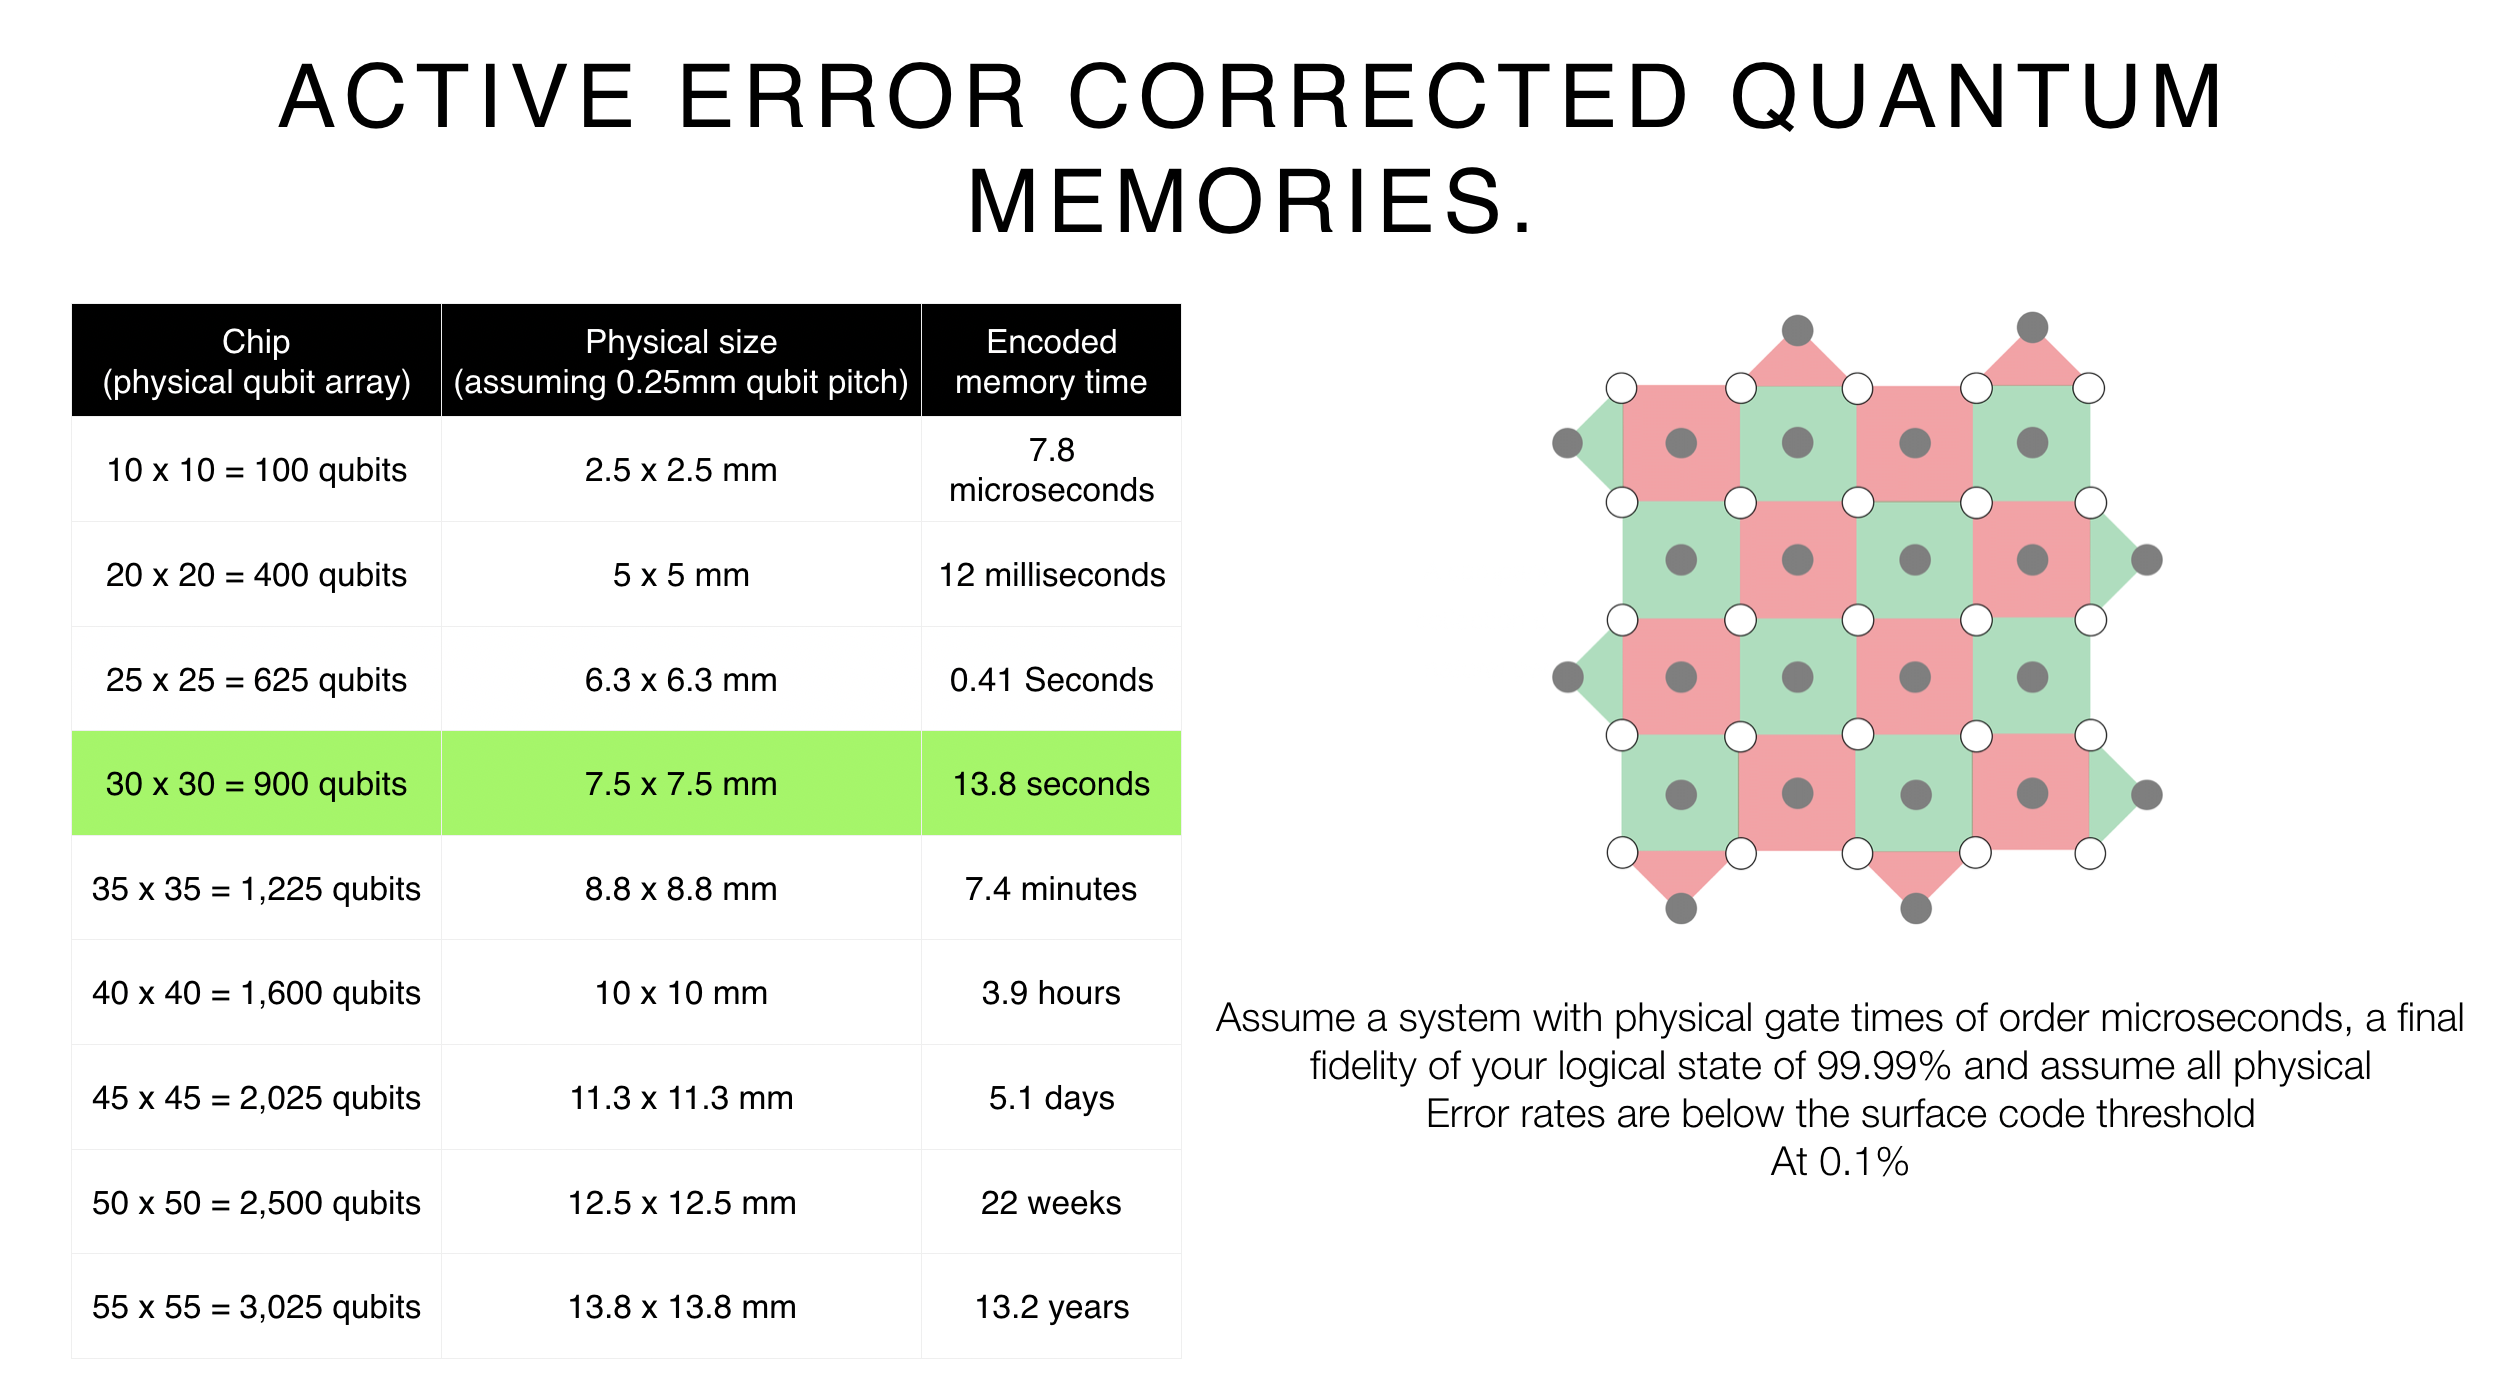
\includegraphics[clip=true, width=0.475\textwidth]{array}
	\caption{} \label{fig:array}
\end{figure}

The physical array of qubits is arranged in a 2D nearest-neighbour connection geometry, wherein individual physical qubits can couple to immediate neighbours to the north, south, east, and west as shown in the right image in Fig.~\ref{fig:array}. 

The surface code has been extremely well studied over the past 15 years. We have extremely accurate simulations that detail the threshold behaviour of the code under a variety of different assumptions and we have quantified very well how the scaling of the code behaves as a function of physical error rate. For this reason we are able to quantify expected \textit{logical} memory time, $T$, in terms of the physical operation time of the quantum gates in our hardware, $t$, the number of physical qubits in the QMU array, $N$, and the logical error rate we want to target, $P$. Through direct numerical simulation, we find:
\begin{align} \label{eq:scale}
T \approx 10t\sqrt{N} P(70p)^{-\sqrt{N}/4},
\end{align}
where $p$ is the physical error rate associated with each of the qubits within each QMU -- assumed to be at least below the Fault-tolerant threshold of the planar code, $p_{th} \approx 0.7\%$.

In the table illustrated in Fig.~\ref{fig:array} we detail the number of physical qubits in a QMU chip, the physical size of the chip-set under the assumption that physical qubits are physically separated by 250$\mu$m, and the amount of time we can maintain the coherence of a single piece of logically encoded quantum information. For this table we assume that physical gates in the QMU chip -- i.e. physical qubit initialisation, measurement, single qubit gates and two qubit gates are all, $t = 1\mu$s. Once the chip set contains approximately 900 physical qubits at a physical dimension of about $(7.5)^2$mm, we can expect to extend the natural coherence time of a piece of encoded information and reliably store it for approximately 14 seconds at a \textit{logical} error of $P= 10^{-4}$.  The performance of the error correction scales exponentially. Consequently, if we roughly triple the size of the chip set, the effective quantum memory time increases to 13 years!

The point where logical information within the QMU can be reliably stored for longer than approximately 1 seconds is the boundary of what we define as \textit{macroscopic quantum memories}. A macroscopic quantum memory is something that can store information long enough to start physically transporting the QMU. Clearly the longer you can reliably store the information in the QMU the further it can be physically moved, but a memory of at least 1 second is needed before you can start doing something interesting using Sneakernet principles.

It should be emphasised that the estimates in Fig.~\ref{fig:array} are based on QEC techniques that are unoptimised for a specific hardware chipset. Performing error correction decoding on a system with biased noise can change resource overheads and it is possible for other QEC coding techniques to be invented that is compatible with hardware engineering constraints that scales better than Eq.~(\ref{eq:scale}) for the rotated planar code. This could reduce the required physical qubit array sizes for a given QMU memory. However, the key message here is that a physical qubit array of on the order of 1cm$^2$, with physical gate times of order 1$\mu$s can be made into very long-lived quantum memories using the same architectural structures and assumptions of quantum computing systems that are already under development (we just require the added property of portability). 

\begin{figure}[htbp!]
	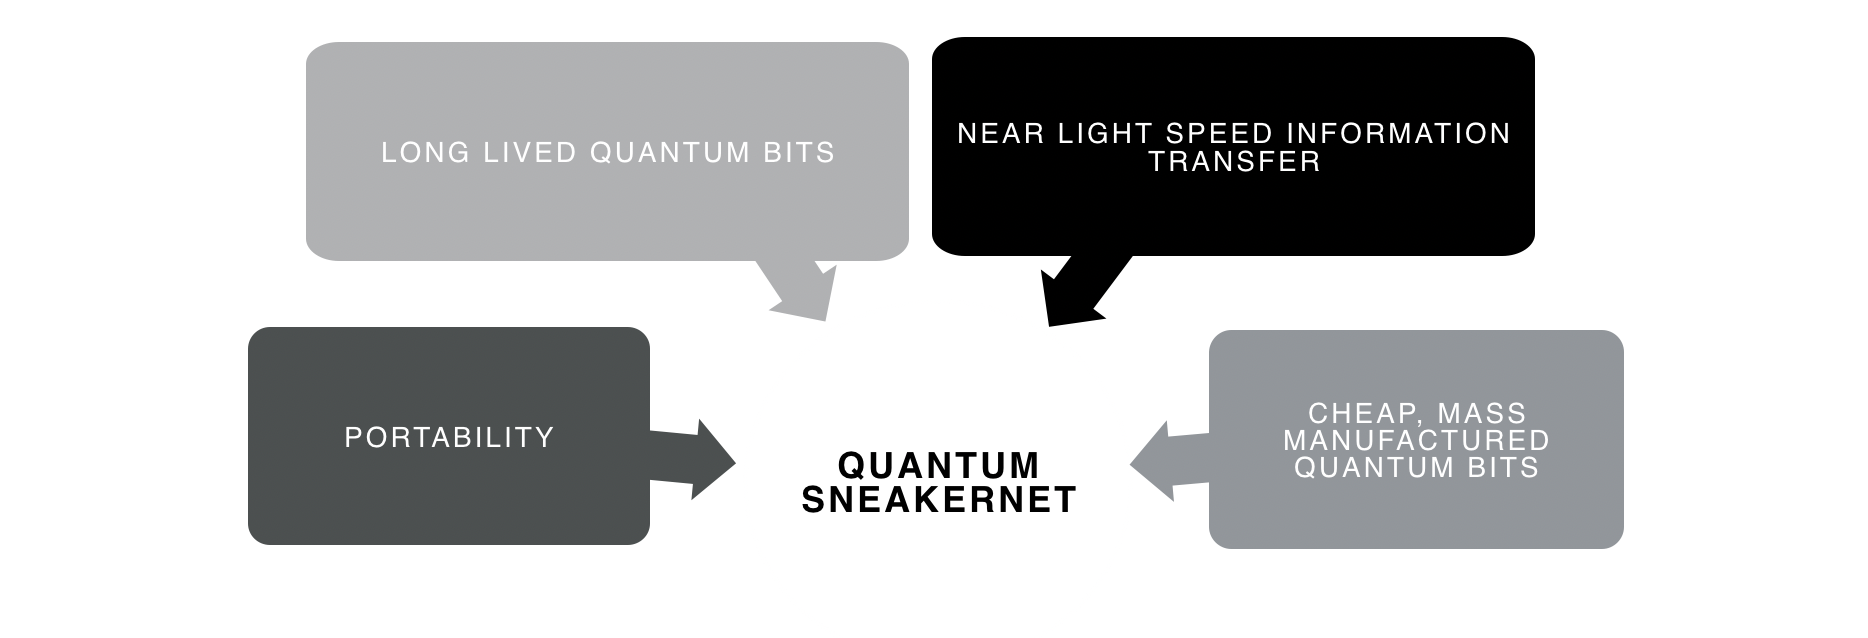
\includegraphics[clip=true, width=0.475\textwidth]{goal}
	\caption{} \label{fig:goal}
\end{figure}

Illustrated in Fig.~\ref{fig:goal} are the four primary technological properties that makes Sneakernet based quantum communications a possible game changer for QKD and global quantum networking. While many are hunting for commercially relevant NISQ \textit{quantum algorithms}, quantum memory units and Sneakernet based communications may be the actual killer application for physical chipsets of the order of 1,000 qubits. However, this will only be of academic interest if systems cannot be be manufactured economically at scale.

\subsubsection{Cheap, mass-manufactured qubit chipsets}

Cost will always be a major issue for any quantum computing or communication/QKD system. While quantum technology opens up a plethora of possibilities in terms of computational power and communications flexibility, it cannot do so with simply a handful of qubits. Unlike the development of classical computation (where the competition for early computers was a room full of people with slide rules) or communications systems (where the state of the art was message exchange using carrier pigeon), quantum technology is competing with an extremely sophisticated and powerful classical infrastructure. 

Many have made the claim that building a quantum computing system or quantum communications network will be akin to other major scientific projects such as the Large Hadron Collider (LHC) at CERN or an array of LIGO gravitational wave detectors for astronomy. However, this analogy is not completely accurate. While LIGO and the LHC are extremely expensive scientific projects, in the case of the LHC there is only \textbf{one} and with LIGO there are only currently \textbf{four} completed operational units. Quantum computing and communications systems will hopefully be ubiquitous in the future. We already know better than to believe, as IBM chairman Thomas Watson reputedly did, `\textit{I think there is a world market for about five computers}'. 

Consequently, being able to mass manufacture physical qubits cheaply will be of paramount concern for any hardware developer in this space. And when we say \textit{cheaply}, we really mean it. Physical qubits in a quantum system are often analogised with physical transistors in a classical information processing system. As you can see in Fig.~\ref{fig:price} the cost of individual classical transistors is \textbf{INSANELY} low. 
 
\begin{figure}[htbp!]
	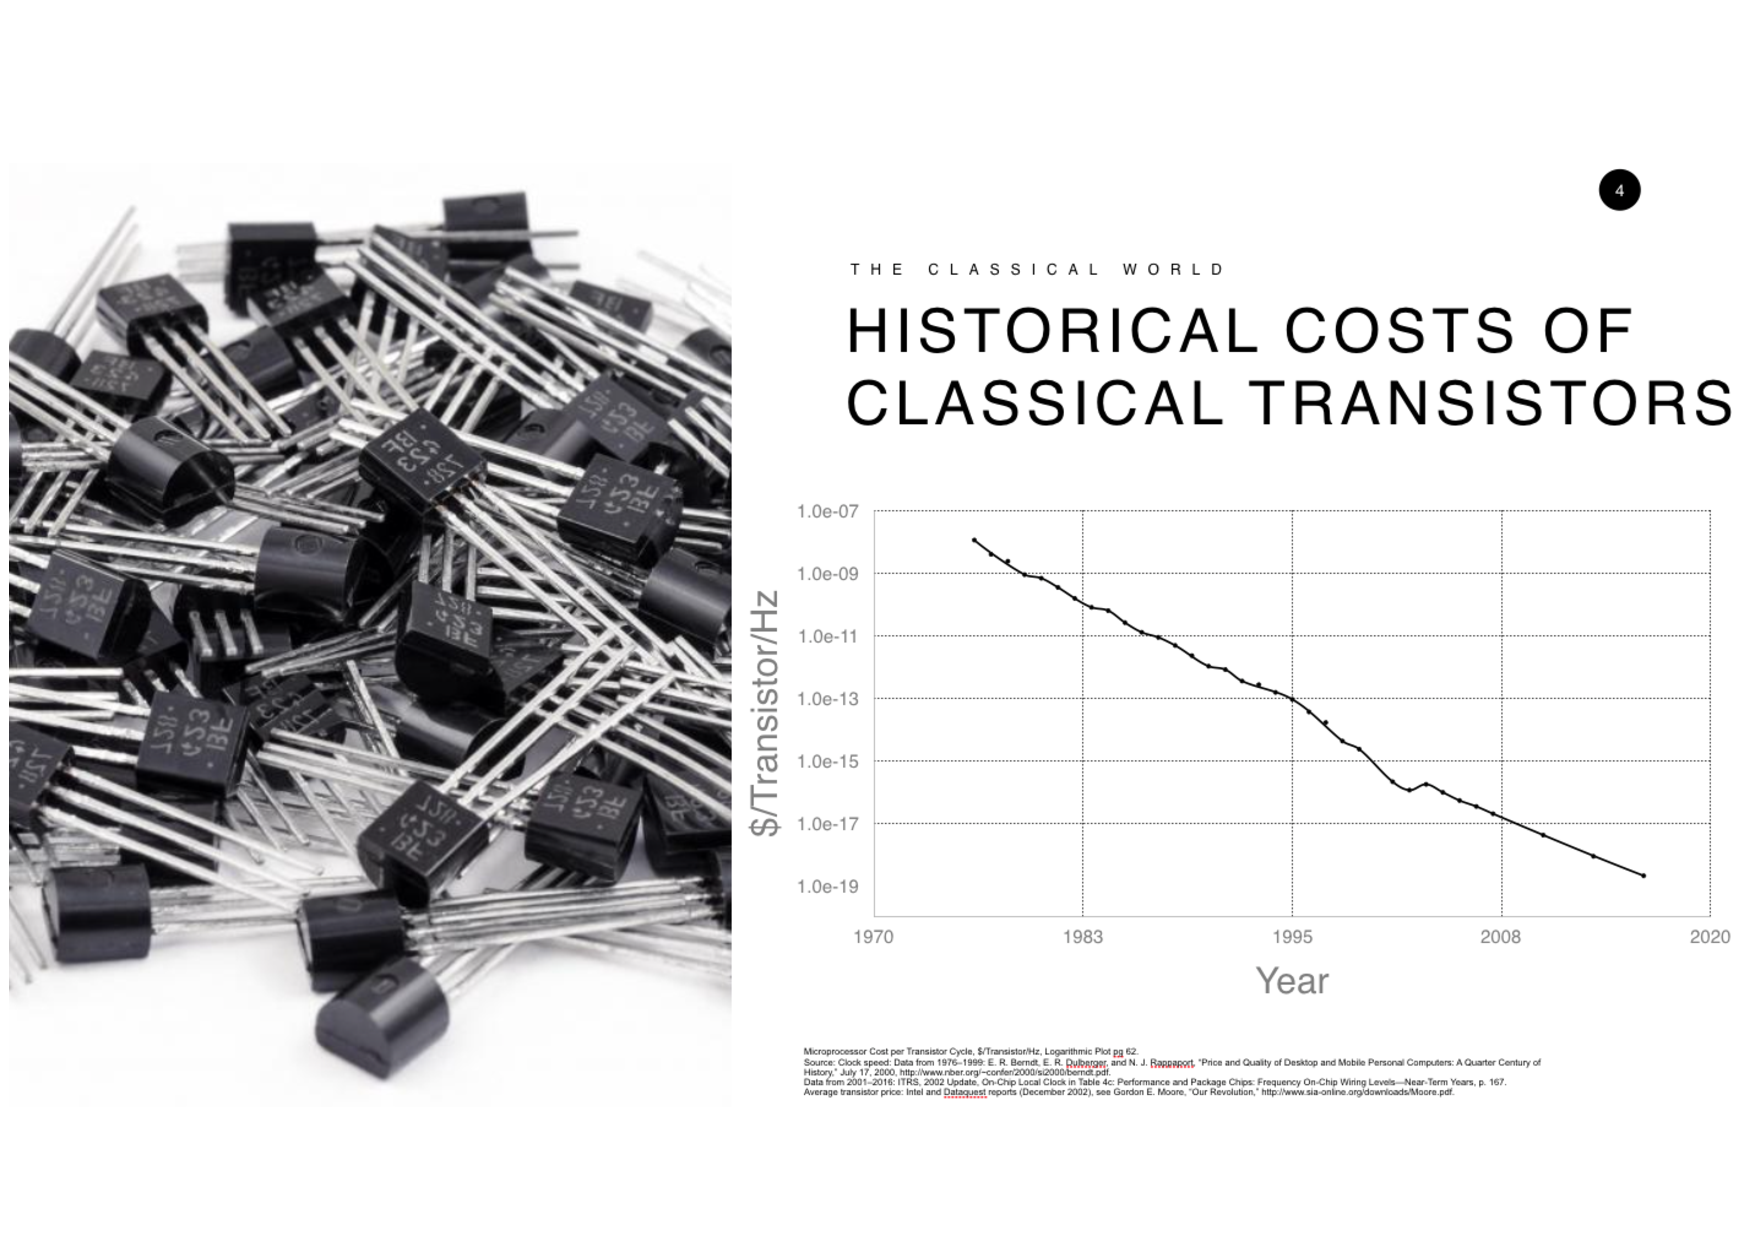
\includegraphics[clip=true, width=0.475\textwidth]{cost}
	\caption{} \label{fig:price}.
\end{figure}

While it is certainly not expected that the price-per-qubit (PPQ) will reach these levels anytime soon, we need to keep Fig.~\ref{fig:price} in mind if we ultimately want to make quantum technology at the scale needed to take full advantage of the power of quantum computing and communications. 

This issue of PPQ is of critical concern for large-scale quantum computing systems. Shown in Fig.~\ref{fig:cost} are costing out of a quantum computing system of sufficient size to perform Shor's factoring algorithm for large key sizes and for quantum simulation of nitrogenase molecules for nitrogen fixation. If an ultimate PPQ goal is not \$1 or lower, there may be little economic motivation for building more than a handful of quantum computers globally. It should be noted that PPQ needs to take into account the infrastructure and control systems as well as the physical qubit itself. For example, in superconducting systems, the required dilution refrigeration system is expensive -- around \$500,000. Additionally, the sample chamber for the dilution refrigerator is quite small in comparison to the `footprint' of a superconducting qubit. A commercial dilution refrigeration system can accommodate perhaps 100 such physical qubits. Consequently, at a minimum, the PPQ in this system would be \$5000.  Additionally Fig.~\ref{fig:cost} does not include any R\&D expenditure or the costs associated with building the fabrication infrastructure to build the qubits themselves. 

All current qubit architectures have associated considerations with regards to ultimate costs of manufacturing a large number of physical qubits and we do expect costs to drop, thanks to economies of scale and efficiency in manufacturing processes as various systems mature. However, we should always keep the \$1 PPQ in the back of our minds as system architectures are invented and experimentally developed. 

\subsection{Operating principles of the quantum Sneakernet}

The basic operational primitive of the quantum Sneakernet system is an old technique for the long range distribution of information. As encapsulated in this wonderful quote from the former director of the University of Toronto Computing Services (UTCS):
\\
\\
\famousquote{Never underestimate the bandwidth of a station wagon full of tapes hurtling down the highway.}{Warren Jackson}
\\
\\
While essentially everyone today is familiar with the principle of classical Sneakernets, many people are not familiar with the name. Rather than sending information via radio waves or fibre optic cables, information it's loaded onto storage memory and physically transported from source to destination. The viability of Sneakernets in the classical world depends heavily on three practical considerations:
\begin{itemize}
\item Availability of cheap, high capacity classical memories
\item Limited bandwidth and high costs associated with radio or optical fibre communications channels
\item The need or lack of need for low latency communications 
\end{itemize}
The first practical consideration for Sneakernet communications has been solved. Classical memories have fallen in price and increased in capacity to an even greater degree than transistor price and density. In 2018, Toshiba released a single 3.5-inch hard disk drive with a capacity of 14 TB available for \$550 USD. 

Let's contrast this capacity with fibre optic connections. In 2016 the new FASTER fibre optic communications link was brought online between northern California and Japan. Costing \$300 million to deploy, it has a total data capacity of 7.5 TB/sec across the Pacific. Consequently, it takes two seconds, utilising the full design capacity of a \$300 million dollar piece of telecommunications infrastructure, to transmit the data contained on a \$550 device that could fit into a handbag. This \$550 hard drive can be shipped via FedEx from northern California to Tokyo for about an extra \$150 and arrive about twenty hours later. Using that approach, we could achieve the same bandwidth as the FASTER network utilising approximately 36,000 hard drives shipped continuously back and forth. The total cost of this would be approximately \$20 Million dollars for the hard-drives and \$5 million per day in commercial shipping costs (which could be made significantly cheaper by using more dedicated cargo transportation systems than FedEx, which is arguably the most expensive).

The capital cost alone associated with the FASTER network is \textit{fifteen} times more expensive than the capital cost of using hard drive-based Sneakernet. The operational costs of the hard drive system would be comparable if not lower than these fibre-optic links. So why do we spend so much time and money on capital and maintenance-intensive classical communications infrastructure such as submarine fibre or communications satellites (Fig.~\ref{fig:classical})?

\begin{figure}[htbp!]
	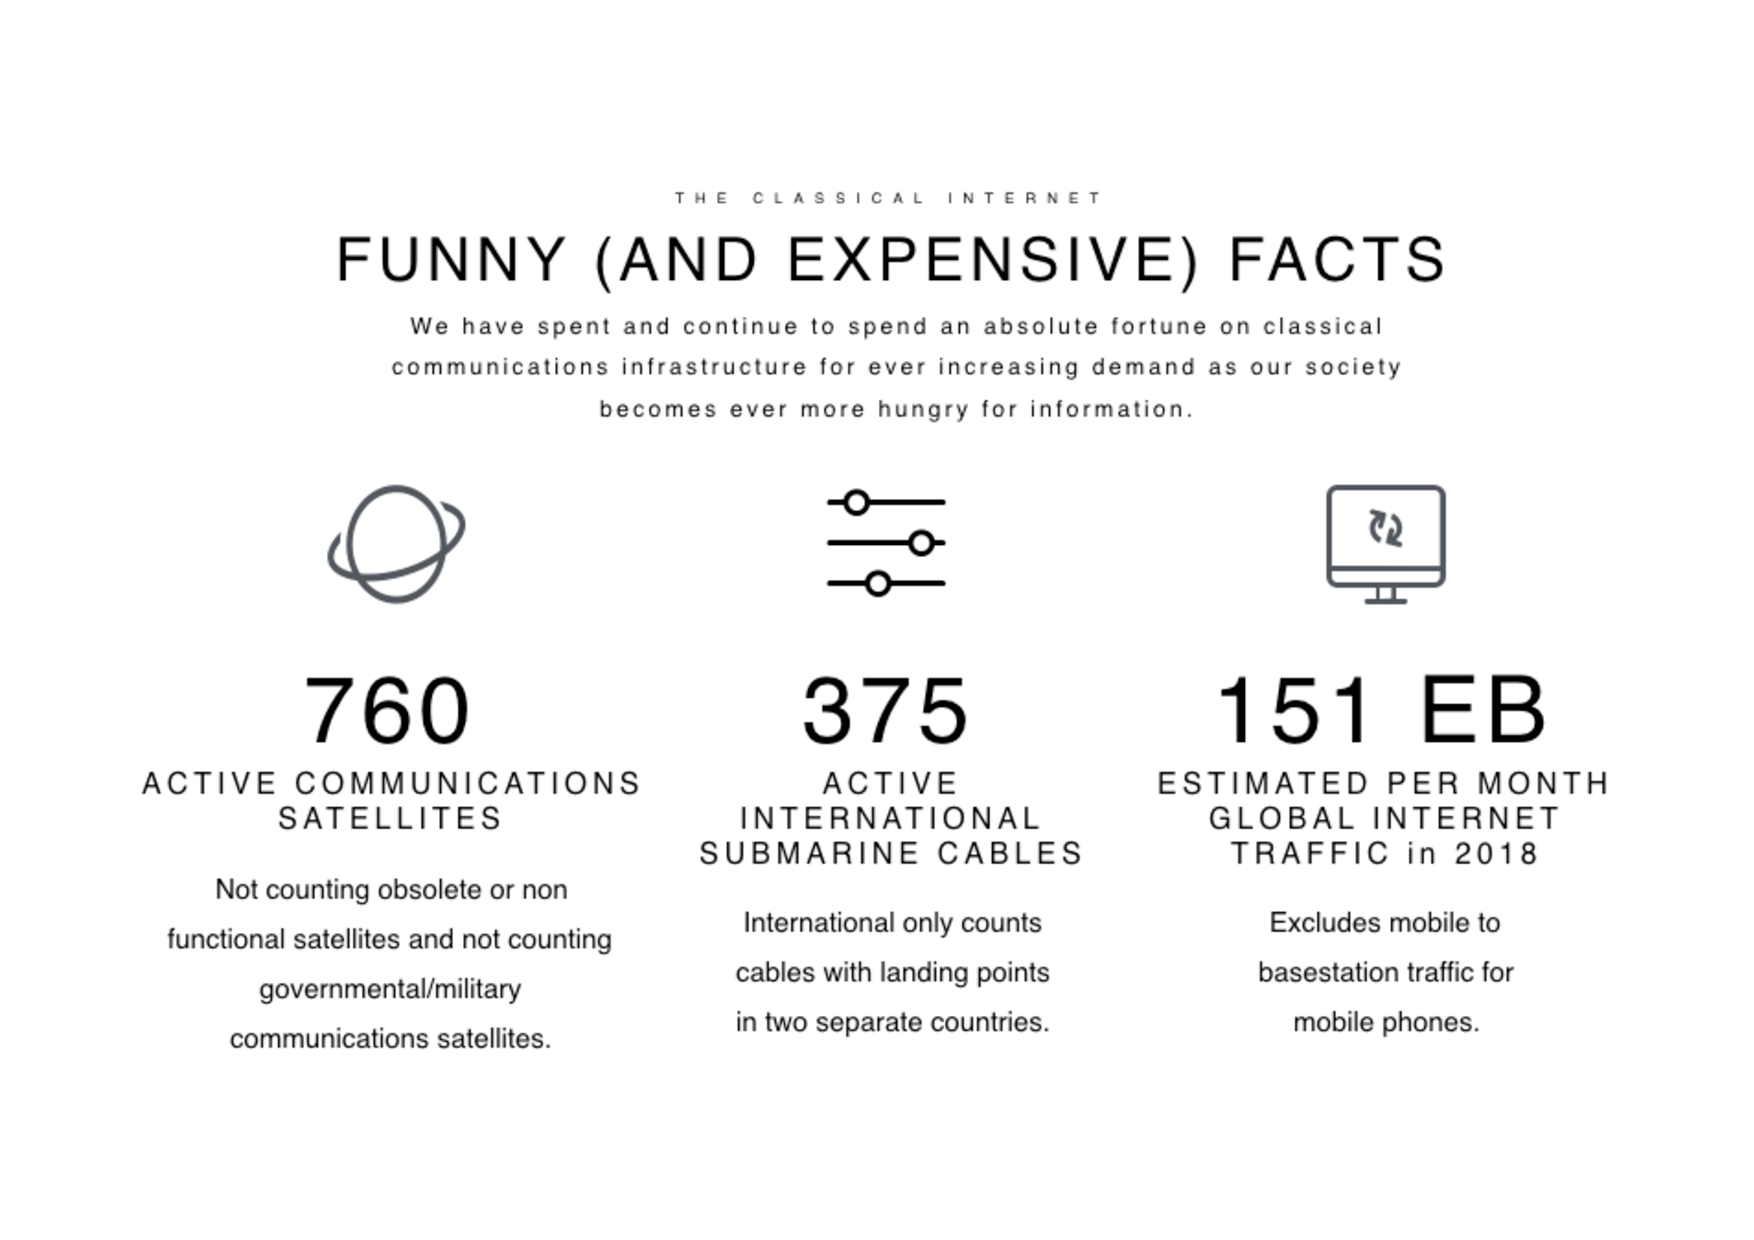
\includegraphics[clip=true, width=0.475\textwidth]{classical}
	\caption{} \label{fig:classical}
\end{figure}

The answer is the third point noted above: \textbf{information latency}. When we transmit information from one side of the planet to another, we don't want to wait twenty hours for the data to arrive. A classical communications system that has that amount of information latency is unusable for most practical applications. Consequently, our classical infrastructure for communications is designed to operate with high bandwidth (capacity) at as close to the speed of light as physically possible. 

Once we move into the quantum regime, we can get the best of both worlds -- the infrastructure benefits of a Sneakernet-based communications link without the latency problem traditionally associated with that approach. 

We can consider a collection of individual QMU's in a single packaged device, forming basically a Quantum memory STICK (QuSTICK). As we have described, a chip set array of physical qubits can maintain and store quantum information for time periods ranging from a day to many decades, depending on the number of physical qubits in the chip set QMU. In Fig.~\ref{fig:array}, a 1.6cm$^2$ chip-set has enough QEC hardware to protect the information for approximately 22 weeks. A QuSTICK consists of hundreds, potentially thousands, of these chip sets in a common cryogenic environment, packaged into a single device would be the quantum version of a USB portable memory stick. However, a classical memory stick and a QuSTICK transport very different things. A memory stick carries classical data; a QuSTICK carries quantum entanglement. This distinction is the key to the power of the quantum Sneakernet. 

\begin{figure}[htbp!]
	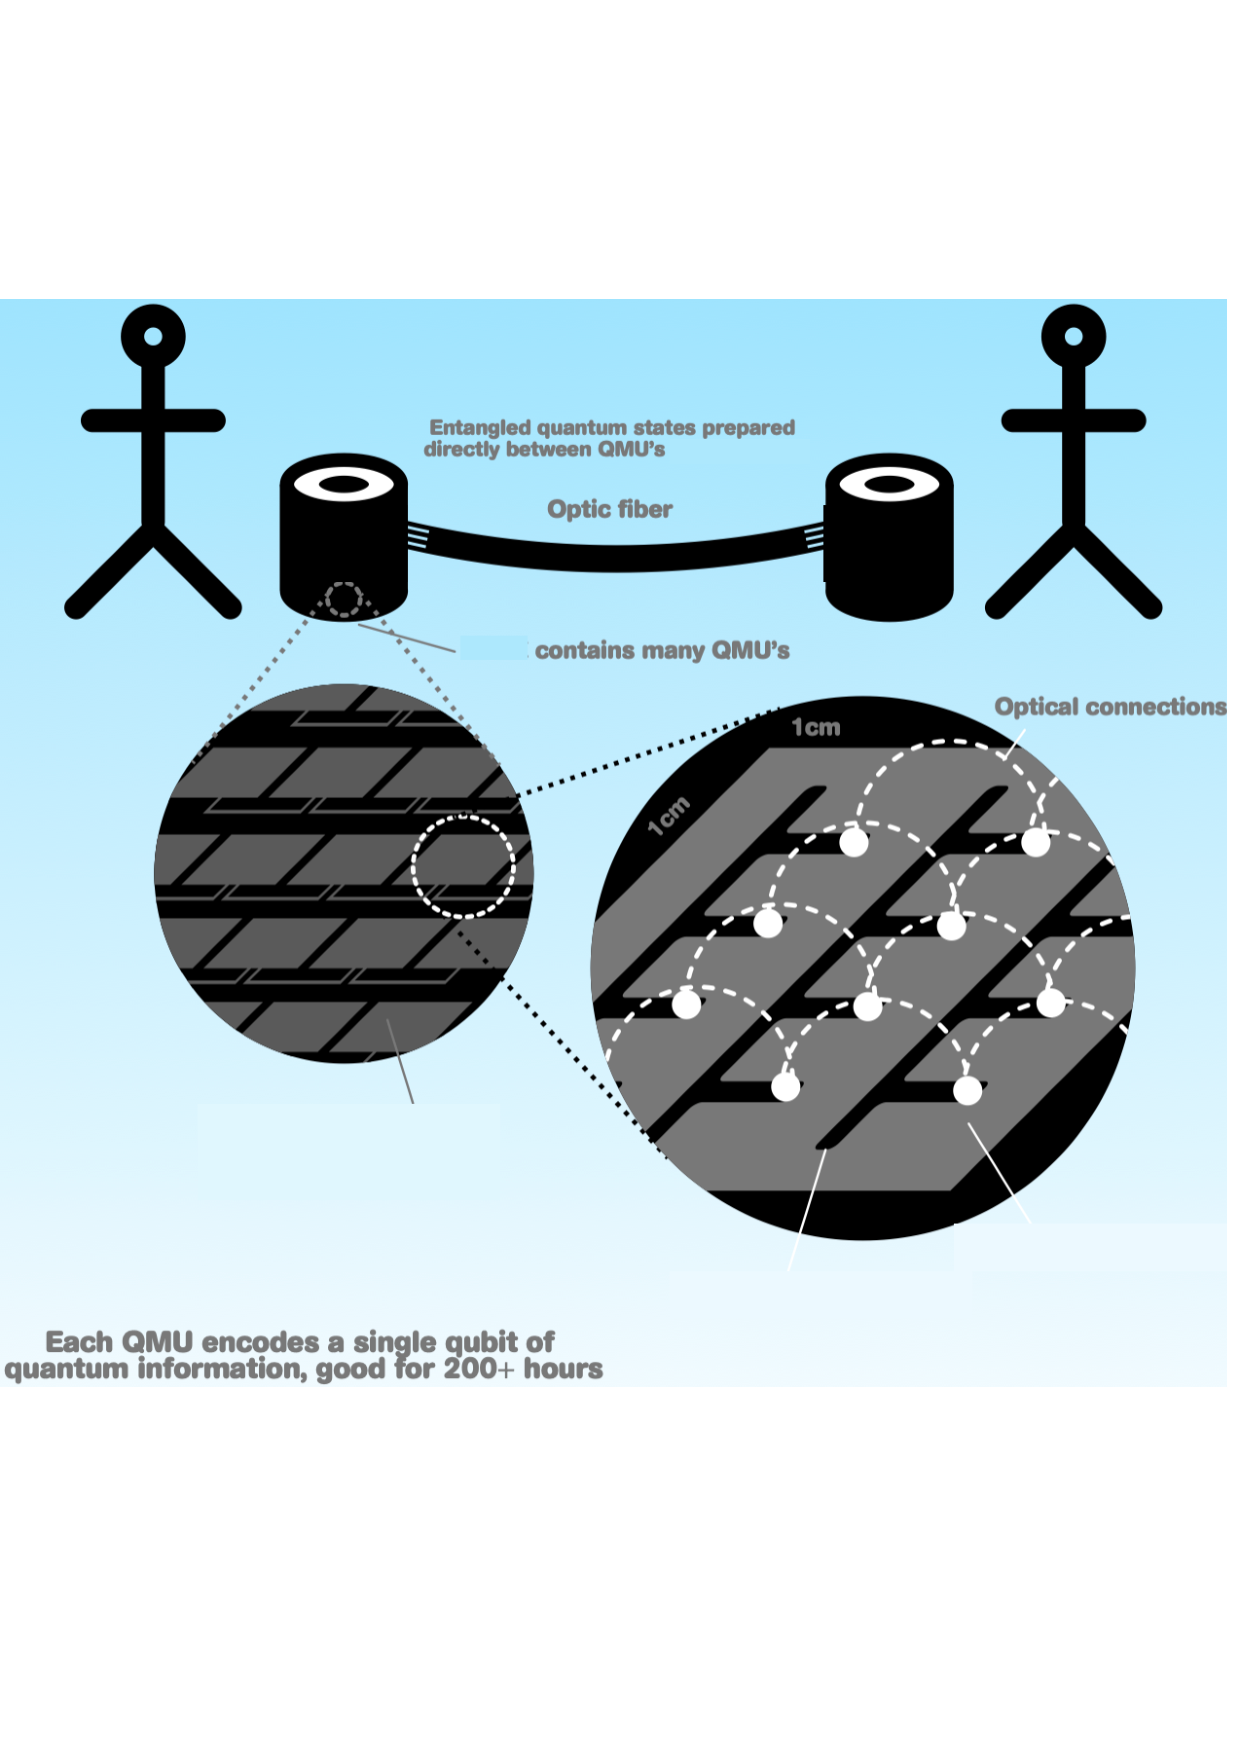
\includegraphics[clip=true, width=0.475\textwidth]{qustick1}
	\caption{} \label{fig:qustick1}
\end{figure}

Shown in Fig.~\ref{fig:qustick1} is the basic structure of the QuSTICK communications link. Two parties, Alice and Bob each have a QuSTICK. The device itself contains multiple Quantum Memory Units (QMU's). Each QMU is chip-set containing sufficient physical qubits to create a long-lived quantum memory of some defined timescale. Referencing back to Fig.~\ref{fig:array}, if the desired memory time is about a day (at a fidelity of 99.99\%), each QMU chipset would consist of approximately 1,600 physical qubits. If we wanted each QMU to protect its respective quantum information for a year, each chip-set would contain approximately 2,100 physical qubits. 

The packaged device would need to contain not only the qubit chipsets themselves, but also all infrastructure required to operate the machine. This may include cooling, laser or microwave control infrastructure, classical computing systems and power. This packaging will ultimately dictate the size of the device and how many individual QMU's could be placed in a single QuSTICK.

\subsection{Transporting quantum entanglement}

Entanglement is a unique property of quantum mechanics that has no classical analogue. Once referred to by Einstein as `spooky action at a distance', entanglement is the ability for quantum particles to remain linked after they have been interacted together regardless of physical separation or physical obstruction. Unless decoherence occurs, there is no evidence that quantum entanglement can be disturbed, blocked or otherwise tampered with. According to the basic principles of quantum mechanics, if two quantum particles are entangled and isolated well enough from the outside world, they can be transported to the opposite sides of the observable universe, with all the stars, planets and black-holes between them, and the entangled correlations will remain undisturbed. It is this entangled state that will be transported by the QuSTICKS. Entanglement isn't information, but rather a quantum resource that can criss-cross the globe and be used as a consumable for quantum related communications protocols such as QKD. 

In Fig.~\ref{fig:array} we illustrated a simple two-party point-to-point connection that is possible with QuSTICKs. Two QuSTICK units, each containing a number of QMU chip sets are built. Each QMU is designed to maintain its integrity for some predetermined amount of time using active QEC protocols built into each QMU. Both QuSTICK units start out in the same room. If physical qubits within a QMU (and between QMU's) are optically connected to each other (if we use colour centres as the underlying hardware technology), it is no more difficult to interact qubits in two separate QuSTICKS than it is to interact qubits that exist in the same QMU. This allows us to create entangled states between QMU's in separate QuSTICKs by simply connecting them together with a suitable optical connection. 

The most basic entanglement protocol is to match up each individual QMU in QuSTICK-1 with a partner QMU in QuSTICK-2 and sequentially create an entangled Bell states between each pair of QMUs. Once this is done, the optic link physically connecting the two QuSTICKs can be removed and the internal error correction will preserve the quantum entanglement up to the time specified by the physical number of qubits inside each QMU.

Each QuSTICK unit has a finite number of QMU's, but there is no limit to the number of QuSTICKs that can be manufactured and deployed in the entire Sneakernet network. For each pair of QuSTICKs we execute this pairwise entangling protocol locally and then then load half of them into a transport vehicle. Shown in Fig.~\ref{fig:loading} is a scenario where a manufacturing factory is `home base' and we are preparing long-lived entangled states with a set of QuSTICKs that remain at `home' and partner sets that are physically moved to different locations. 

\begin{figure}[htbp!]
	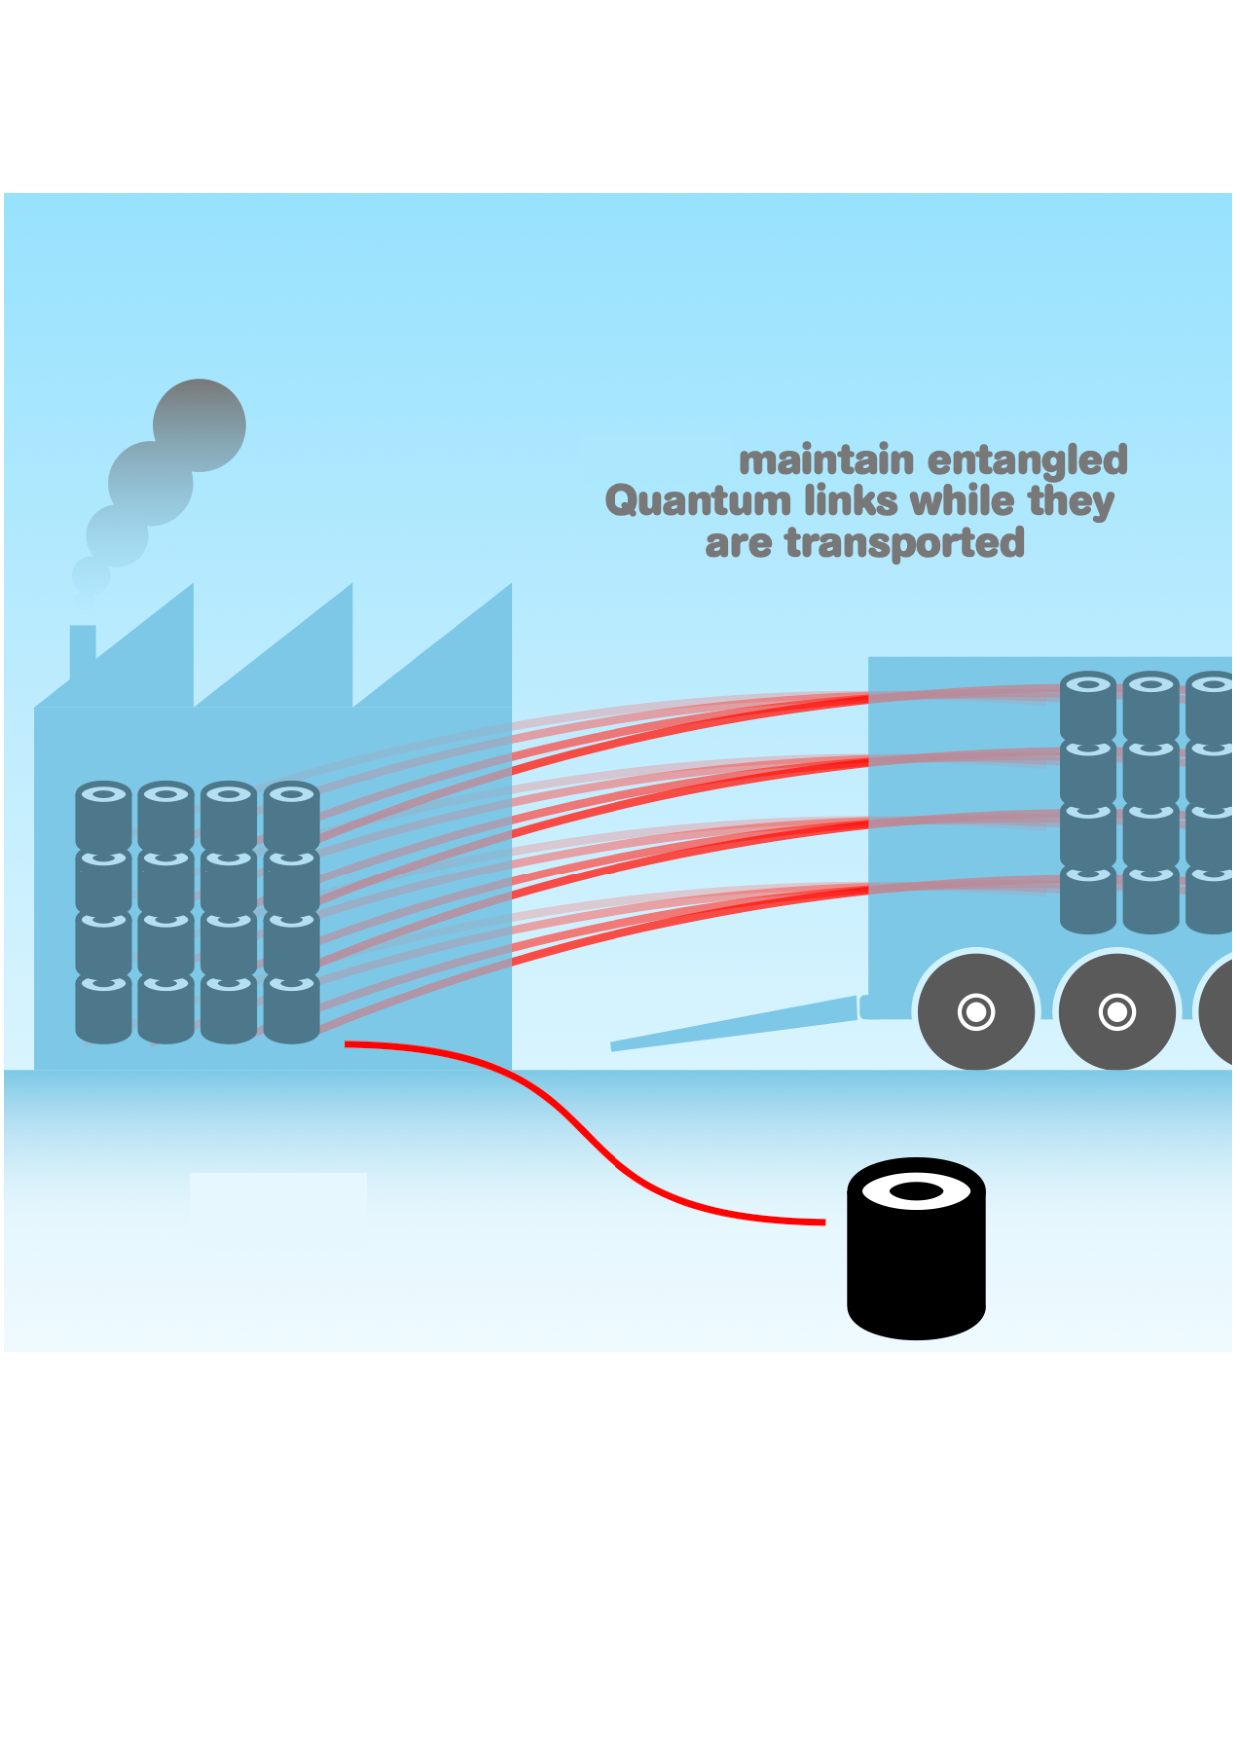
\includegraphics[clip=true, width=0.475\textwidth]{qustick2}
	\caption{} \label{fig:loading}
\end{figure}

It is important to note that when the entanglement is initially prepared, we do not need to know the destination of the transported QuSTICKs or their eventual application. The application could be highly sensitive QKD distribution or it could be a very public scientific experiment. The only thing we care about is that the QMU's inside each QuSTICK have sufficient quantum memory time to get to their destination with their entangled state intact at the desired fidelity.

Once the entanglement is prepared, the entanglement links are \textit{automatically} preserved while the devices are being physically moved. The internal error correction protocols for each QMU ensures that errors produced by the physical qubits themselves or the act of physically moving the system are effectively corrected. The portability of the architecture is crucial to this. 

Not all QuSTICKS have to go to the same destination. Once the entanglement is prepared at home base, a subset of QuSTICKS may be transported to destination A, another subset to destination B and so on. In fact, destination A may be 5km up the road, while destination B is half way around the world. Destination C might use low-cost cargo shipping to receive their QuSTICKs, while destination D's need might be for fewer units sooner, and so shipment by air is preferred (as shown in Fig.~\ref{fig:distribution}). The flexibility enabled by portable quantum memories allows for dynamic allocation of both QuSTICK resources and the use of whatever physical transport method is appropriate to support the final application. This is in contrast to the 'one size fits all' approach used by infrastructure-intensive communications systems like satellites and repeaters. Such systems operate in exactly the same way regardless of the demands of the ultimate application.

\begin{figure}[htbp!]
	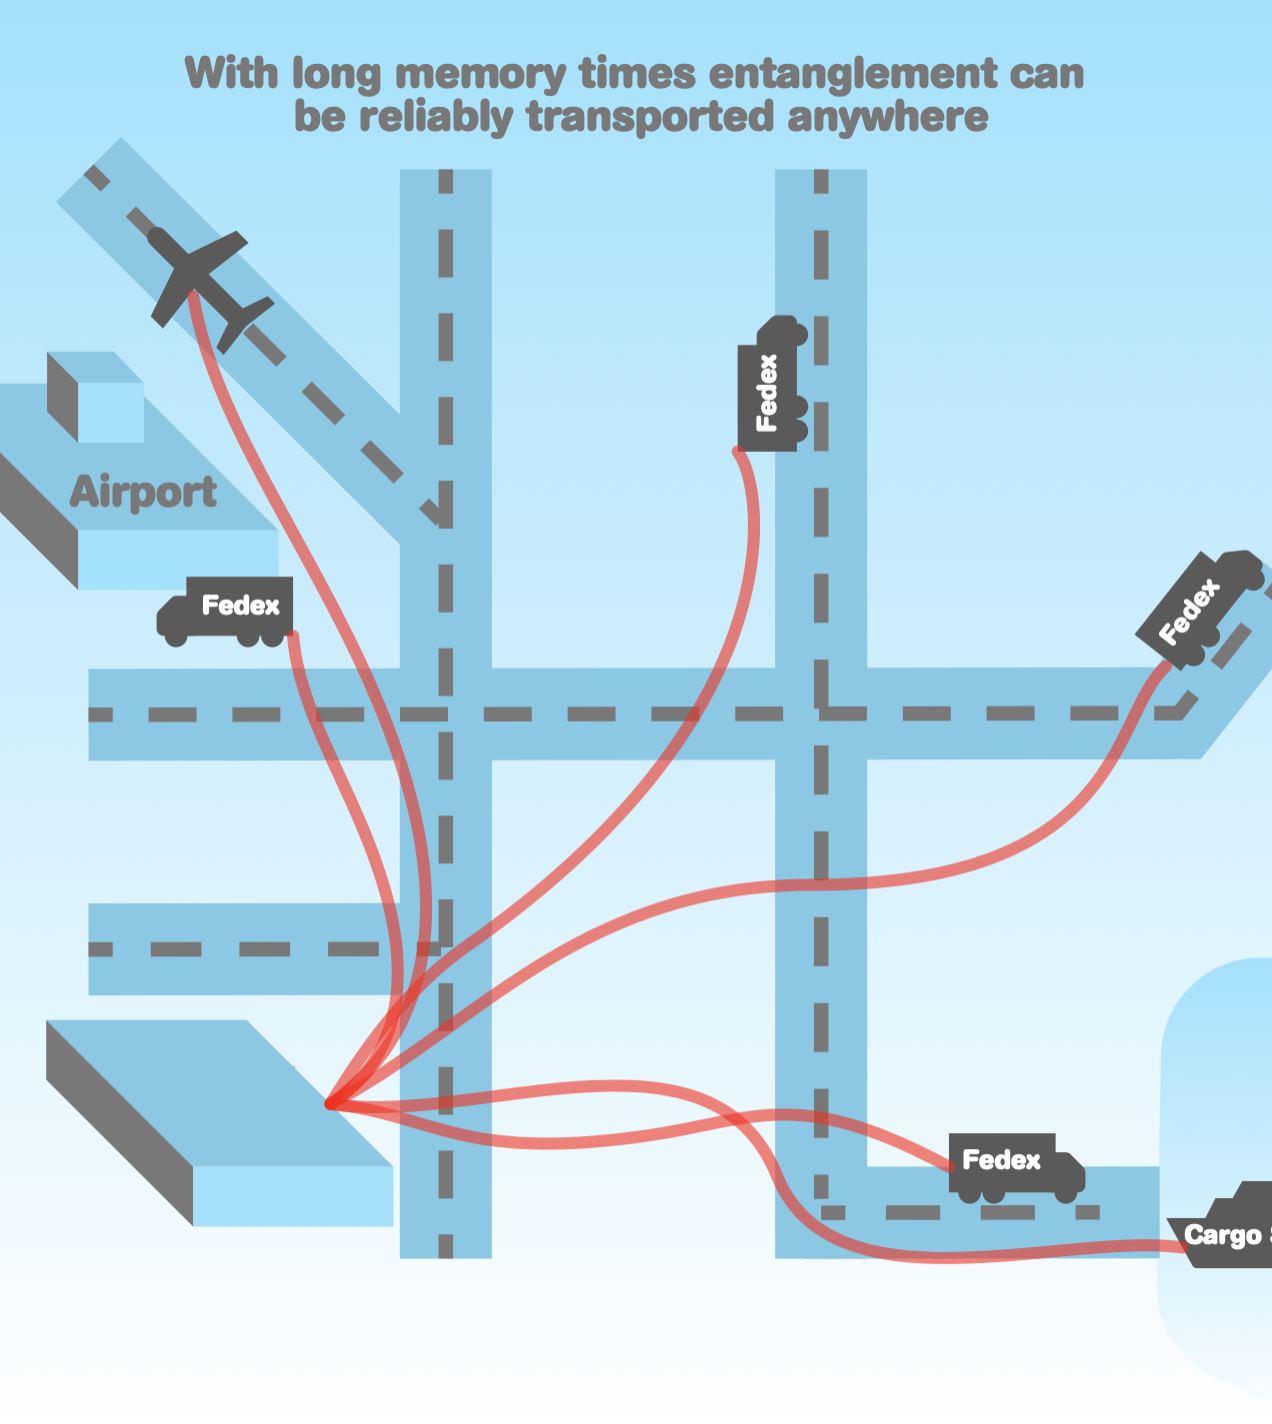
\includegraphics[clip=true, width=0.475\textwidth]{qustick3}
	\caption{} \label{fig:distribution}
\end{figure}

\subsection{Using and re-charging QuSTICK quantum entanglement}

We have described a system where a finite amount of entangled quantum states is maintained by a set of QuSTICKs for a predefined period of time. This period of time needs to be sufficient to entangle the QuSTICKs directly together at the source and physically transport them to the destination. This mechanism now mimics the behaviour of a quantum satellite or quantum repeater system, but with a crucial difference that ultimately makes the Sneakernet system superior from a practical standpoint:
\begin{itemize}
\item The sender and receiver now share a persistent, high fidelity entanglement link that \textbf{does not have to be used immediately}. Quantum satellites and ballistic repeater designs generate entanglement using photons. They are not designed to `store' the entanglement for future use -- the entanglement needs to be consumed for some type of communications protocol immediately upon receipt.
\item The total amount of entanglement a destination shares with home base is dependent only on the number of QMU's and QuSTICKs used. If only 100 entangled states are needed for an application, a single QuSTICK (containing 100 QMU chips) will suffice. One million entangled states would require 10,000 QuSTICKS at 100 QMU's per stick. 
\item The entanglement the Sneakernet provides is \textbf{by design} ultra-high-fidelity. All of the numbers in Fig.~\ref{fig:array} assumes that each QMU can maintain an encoded piece of quantum information for a given period of time \textbf{to a fidelity of 99.99\%}. Increasing the fidelity even further requires only a small increase in the size of the QMU. If a target application requires a fidelity of 99.999999999\% (say for direct connections between fully fault-tolerant quantum computing systems), simply use a few more physical qubits per QMU. i.e. a $T= 22$ week QMU at 99.99\% fidelity requires 2,500 physical qubits, the same $T=22$ week QMU at 99.999999999\% requires 5,400 physical qubits. That's just over double the physical size for 7 orders of magnitude increase in fidelity.
\item Sneakernet entanglement connections can reach global distances (Alice's QuSTICK in Sydney can be connected to Bob's QuSTICK in London using conventional transportation services).
\item The persistent entanglement shared can continue to move before it is used. Alice may not want to use this entanglement in Sydney, but instead transport it to central Australia. The entanglement link with London will continue to move with Alice as long as her QuSTICK provides sufficient error-correction for the additional time required.
\end{itemize}

\subsection{Entanglement swapping}

Another extremely beneficial aspect to the quantum Sneakernet design is the ability to \textbf{SWAP} entanglement. What does this mean? 

In Fig.~\ref{fig:distribution} we assume that all QuSTICKs that will be physically transported are initially physically connected to partners sitting at their home base. This creates a star-network structure, where the home base acts as an endpoint node for all of the entanglement links that are physically distributed outwards. But suppose two distributed QuSTICK units want to share entanglement directly? Do they need to physically meet and have their optical links hooked up? No, instead they can ask for an entanglement SWAP protocol to occur. 

Let us take three parties: Alice, Bob and Alan. Alan is located in Berlin, and, as in the previous example, Alice is in Sydney and Bob is in London. In total there are four QuSTICKs. Alan has initially manufactured all four, and we will call them ALICE, BOB and ALAN-(1,2). Before putting ALICE and BOB onto airplanes or ships, Alan entangles all of ALAN-1 QMU's to the QMU's in ALICE, and similarly between ALAN-2 and BOB. ALICE and BOB are then shipped off to Sydney and London respectively. Again, at this point, nobody has decided exactly how they are going to use this entanglement; but (depending on the amount of memory time provided by each QMU in each QuSTICK) they have a fixed time during which they can use it for anything. 

Once ALICE and BOB arrive, Alice and Bob only share entanglement with Alan directly. However, at some point, Alice and Bob decide that they want a direct entanglement connection with each other (for example, if they are intending to establish some cryptographic keys).

Instead of physically moving again, Alice and Bob can request an entanglement SWAP from Alan. Alan will then connect ALAN-1 and ALAN-2 directly together (since he still has physical possession of both units in Berlin) and entangle each of their QMU's. If Alan then measures each of the QMU's in his two QuSTICKs in the $X$-basis, the entanglement he initially shared with Alice and Bob is SWAPPED to them. By performing this operation, Alice and Bob can share \textbf{directly} two QuSTICKs of entangled QMU's without ever having to physically meet each other. They can then proceed to perform whatever communications protocol they wish. This SWAPPING protocol is illustrated in Fig.~\ref{fig:SWAPPING} 

The above example highlights an important point. The physical distribution of a set of QuSTICKs creates an \textit{initial network topology} for their entanglement. However, this topology can be modified after the fact to create direct entanglement connections between parties that were never initially in the same distribution channel. The physical distribution network can be thought of as a network graph. Initially, each node is the physical location of a QuSTICK, and each edge connects the node where a QuSTICK began its journey to a node where it ended its journey. Entanglement SWAPPING allows us to change the structure of the graph (i.e. change where edges are and are not) without having to move the QuSTICKs again. 
 
\begin{figure}[htbp!]
	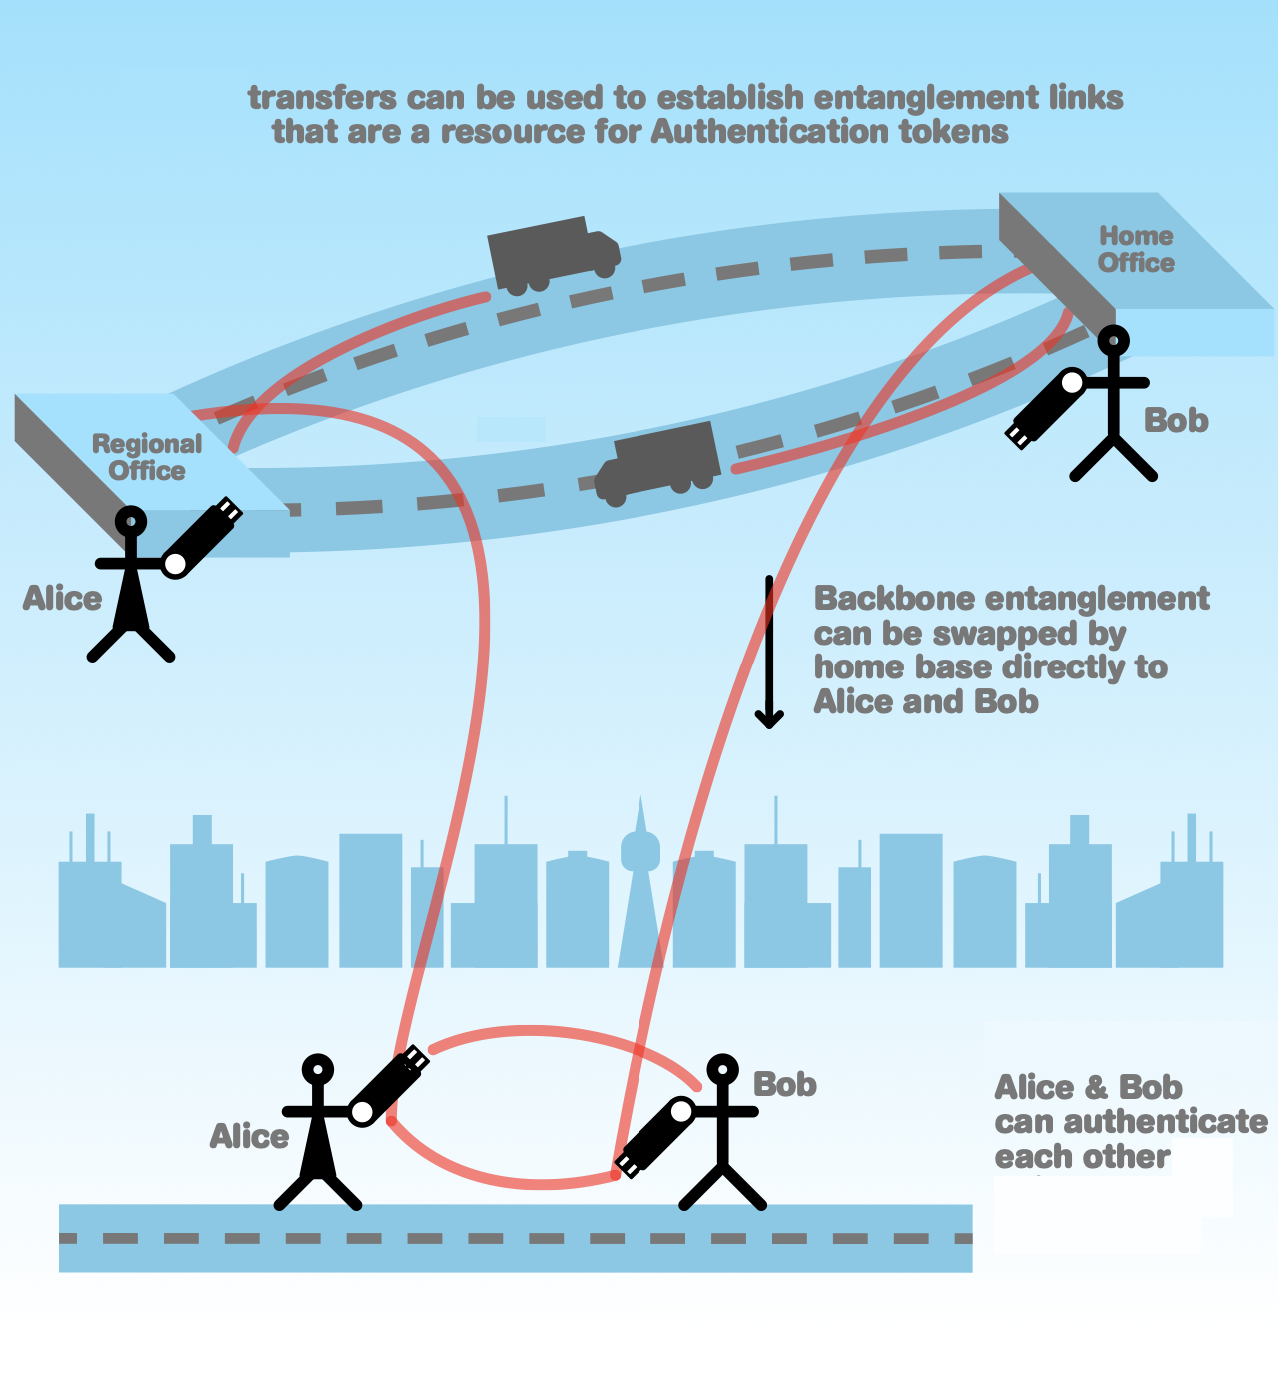
\includegraphics[clip=true, width=0.475\textwidth]{SWAPPING}
	\caption{} \label{fig:SWAPPING}
\end{figure}

This kind of flexibility is simply not possible in classical networking design. It would be as if a classical data packet could be sent \textbf{directly} between the Australia and Iceland despite there being no direct telecommunications link between those two countries. Classically, the data packet would have to first travel from Australia to Singapore, then perhaps from Singapore through routers in west Asia, the Middle East, central and northern Europe, the U.K. and finally to Iceland. At any point in its journey the packet might be intercepted, copied, lost, tampered with, inspected, corrupted, or accidentally routed to a completely inaccurate destination. 

With entanglement SWAPPING using the Sneakernet network, we can define a network topology first, before it is used, and then later define direct entanglement connections between parties that were never in direct physical contact. This opens up a whole new world in network design theory. 

\subsection{Entanglement depletion \& network persistence}

The use of the entanglement that is prepared between two parties to actually perform a given communications or computational protocol generally consists of the following broad steps: 
\begin{itemize}
\item The parties to the protocol first configure the entanglement network, through SWAPPING, to match the requirements of the protocol.
\item Each party measures the \textit{logical state} of each QMU by physically measuring every physical qubit that QMU comprises. These measurements can occur in many different ways (technically referred to as the \textit{basis} in which the logic state is measured). Measuring a logic state in each QMU results in a yes/no answer. Choosing a different \textit{basis} to measure the QMU is akin to asking a different yes/no question. 
\item The parties in the protocol announce, publicly, over a classical communication system, what \textit{QUESTION} the QMU's are being asked. i.e. each party only announces the BASIS they chose to measure their respective QMU's in. They never reveal the ANSWER the QMU's gave. 
\item All the classical \textit{ANSWERS} between the QMU's are now completely correlated due to the initial quantum entanglement the parties shared. 
\item The entanglement carried by each QMU has now been destroyed or \textit{consumed} to perform the protocol and is no longer present to use again (although, of course, the QuSTICK itself isn't affected and can be re-entangled any number of times). 
\end{itemize}

What happens when the collection of QMU's within a QuSTICK has been depleted? The entanglement resource of a QuSTICK is analogous to a battery that carries a fixed amount of charge. A battery is a physical unit that can be used in many different ways and moved around to different devices; but it contains a resource that is finite. Once that finite resource has been exhausted, it must be replenished again from an appropriate source. In the case of a battery, it's recharged from via electrical outlet. In the case of a QuSTICK, the replenishment comes from another QuSTICK.

A fabrication factory may be the source of the physical QuSTICKs, but is not, in general, the source of entanglement. Returning to the battery analogy, the Tesla's Gigafactory may be the source the physical batteries, but it isn't the source for the battery \textit{energy} in your Tesla vehicle. 

Network connections between QuSTICKs can be established whenever and wherever QuSTICKs can be physically connected to each other. And, as discussed above, via SWAPPING protocols, entanglement connections can be reconfigured over very long distances. While the system is certainly designed to be portable over global distances, we can also exploit the `small-world phenomenon' to construct long range entanglement with only relatively short physical movement of QuSTICKS. 

Once the entanglement in a QuSTICK is consumed and depleted, the owner or operator of the QuSTICK simply has to physically find another QuSTICK that has some entanglement `charge' left. If Alice has no entanglement left, she could go find Charlie (who hasn't consumed his entanglement yet) and physically connect her QuSTICK to his and re-entangle all the QMU's. At this point, Alice has reentered the entanglement network. Once she has, she can use SWAPPING to establish connections to another network member to perform more communications protocols. There is no need for her to reconnect to a central entanglement hub or a distant source that would require her to ship her QuSTICK to the other side of the planet and wait for it to return. 

Entanglement is a consumable resource. But, unlike a battery, the entanglement `charge' is a free resource that comes as a consequence of two QuSTICKS being in the same room. 

The processes described above enable a persistent network to exist. Even though users will consume QuSTICK entanglement whenever they use their device to perform a quantum communications protocol, that networked entanglement can be replenished easily. Again, the nature and structure of QuNET allows us considerable flexibility in network topology. We can essentially design a two-stage embedded network: One stage in which the structure of the network is determined by the physical interaction of the users who have access to physical QuSTICKs, and a second stage in which quantum information flow is dictated by the structure of the underlying entanglement network. This is inconceivable in the classical world of information networking. We can only begin to imagine what remarkable things are possible with this kind of technology infrastructure. We can be certain that it will unlock capabilities well beyond the basic ultra-high security quantum communications applications that we are discussing here. 

\subsection{Quantum Sneakernet protocols}

Many different communications protocols can be enacted using QuSTICK entanglement and the Sneakernet. The principal determining factor for what can be done with this technology is the number of units that can be physically manufactured and deployed. As production increases, and the total number of QuSTICKs in the world grows, new communications applications become possible. One of the major benefits of a Sneakernet design is that \textbf{the entire network is expandable}. We don't replace a QuSTICK every time we a new one is manufactured; we simply add it to the network to increase overall capacity. Generation one of the QuSTICK design will be compatible with future generations. New design iterations will primarily increase quantum data capacity (as is the case with classical memory chips), and a QuSTICK-based communications network will become more complex, higher bandwidth and more flexible as additional QuSTICKS are deployed. 

A central principle (violation of Bell's Inequality) underlies each of these protocols, and the non-specialist reader may want to take a moment to review the fundamentals of quantum entanglement and its utility in secure communications throughout the rest of this book. These discussions will be largely qualitative as the main take away points is the flexibility that a Sneakernet based network allows for when realising detailed communications protocols that have been analysed extensively in other chapters. Most of this quantitative analysis for these protocols talk about the number of entangled bits (or eBits required). In our discussion, eBits are equivalent to a pair of QMU's within a pair of QuSTICKS. 

\subsubsection{Authentication protocols}

An authentication protocol is generally a small data-exchange mechanism used to confirm that a user is who he says he or she is, and that the information that is to follow will not be coming from a third party or impostor. It is used extensively in classical communications for applications that range from the routine (when I go to www.google.com, am I really talking to Google?) to communications that determine the survival of the human race (did the launch order received by an Ohio-class nuclear submarine really come from the White House?) In a Sneakernet based communications system, authentication tokens will be one of the first applications due to the comparatively small number of QMU's needed. 

The key question that the authentication process must answer is this: How do we ensure that messages are coming from the requisite trusted source? Turing's solution is similar to physical authentication tokens that some bank customers are given to access their accounts for high-value transactions. These classical authentication tokens utilise a variety of methods to ensure that the server (e.g. a bank website) and the client (the person with a bank account) can share a secret message that can be used to authenticate a log-in session. Some utilise static password tokens, some use synchronous dynamic tokens and some use a type of `call and response' method. There are even services that use a smart phone APP to verify the phone's SIM card and then generate a one-time key. All of these techniques are vulnerable to security flaws that present themselves if: 1) the implementation is not done perfectly, 2) the token is lost, stolen, or duplicated, or 3) if some classical calculation that was assumed to be computationally difficult is compromised in some way. 

A quantum Sneakernet solution uses the same basic principle as the classical authentication token -- the client and server share a physical object -- but, because our QuSTICK units are quantum in nature, we can use the laws of physics to ensure complete security of the authentication protocol. The underlying idea is that two parties, Alice and Bob, can violate a Bell inequality if and only if they share an entangled Bell state. That is, two QuSTICKs that are entangled will behave differently when queried than two QuSTICKs that aren't entangled.

To illustrate the protocol, we stipulate that our two parties share a finite number of Bell states between them, with one half of the Bell states contained within Alice's QuSTICK and the other half within Bob's QuSTICK. This shared Bell state will typically be prepared ahead of time in QMU's inside a QuSTICK system by a third party and then distributed to Alice and Bob. That is, Alice and Bob have received their respective halves of the entangled state from some other QuSTICK source of entanglement. The source could be a much larger backbone quantum network that is distributing long-range entanglement via the SWAP mechanism as described in the previous section. Alternatively, the physical QuSTICKS themselves could have been delivered to Alice and Bob by a third party or parties. However, as we will see below, this third party source of QuSTICKs or entanglement does not need to be trusted by either Alice or Bob.

If Alice and Bob share Bell states between each other, then they can perform a \textit{Bell violation test}. We will briefly summarise the basic test below. In a nutshell: The Bell parameter, $S$ is calculated by performing measurements over a finite set of shared Bell state. In classical theory, this parameter, $S$ must be $\leq 2$, while in quantum theory, $S=2\sqrt{2}$. Hence to confirm that Alice and Bob indeed shared a quantum state, we must determine if $S>2$.

Using a standard error analysis, for $M = 100$ shared Bell states between Alice and Bob, the standard error is approximately 0.4, implying that with 99\% confidence, $S > 2$. Hence 100 QMU's in each of two entangled QuSTICKs can be used to violate a Bell inequality with very high confidence, guaranteeing (assuming that quantum mechanics is correctly describing the behaviour of the QMUs) that Alice and Bob do actually share entangled states. Each QuSTICK is designed to distribute extremely high fidelity Bell states, and any possible hardware or implementation inaccuracy is addressed with the internal error correction of each QMU. As a result, the primary source of error in this example is sampling error.

The portability of QuSTICK units is what drives many of the potential applications of this design. While 100 error-corrected QMU's is a large number compared to what is currently available, The system is designed to scale to this level almost immediately. The long-lived nature of our QMU's and QuSTICKs -- and the ability to move them anywhere -- allows for deployment of these units across a wide range of platforms and environments. 

Whenever ultra-high security is needed, particularly for message authentication, the Sneakernet is particularly valuable. The fact that quantum entanglement is prepared locally, at home base, before any of these units are physically deployed in the field adds tremendous security benefits. Such benefits are not available with quantum protocols based on the transmission of the entangled pairs. Why? To put this a different way: It is very difficult to detect if an eavesdropper is trying to steal a photon from an optical fibre or a photon flying through the air. It's a lot easier to know if someone has hit you over the head and stolen your QuSTICK!

As quantum entanglement is not obstructed by any known physical process, the links provided by the QuSTICKS cannot be disrupted or destroyed unless someone has physical control of the QuSTICK units themselves. Provided an unencrypted communications channel exists that allows communication with Alice and Bob for reconciliation, QuSTICKS can always be used to perform secure authentication. 

QuSTICK-based message authentication will likely be the initial application of a Sneakernet based quantum communications platform as it can occur with a small number of QMU's and hence physical qubits. However, the system is adaptable. Initially, while QuSTICKS are sparse, we can run the Sneakernet system as simply a network for secure authentication. As we fabricate and deploy more QMU's and QuSTICKS, the authentication network grows until we hit a critical volume of devices, at which point they can be re-tasked to more complex quantum communications protocols, and the growth cycle starts again. Ultimately, as QuSTICK volume increases, we can run authentication protocols, QKD protocols, distributed quantum computing and communications and anything in between over a shared network that does not require segregated sub-networks for highly secure applications. 

\subsubsection{Key exchange}

The next step after authentication protocols is key distribution using standard QKD protocols and additional QuSTICK units. 

The QKD literature is now very rich, so we won't go into as much detail on how QKD can be implemented and optimised. The basic process involves distributing a shared random bit-string that can be used to encrypt messages using strong, symmetric classical cryptographic protocols. In the most current, declassified standards, the U.S. National Institutes of Standards and Technology (NIST) states:

\textbf{The design and strength of all key lengths of the AES algorithm (i.e., 128, 192 and 256) are sufficient to protect classified information up to the SECRET level. TOP SECRET information will require use of either the 192 or 256 key lengths. The implementation of AES in products intended to protect national security systems and/or information must be reviewed and certified by NSA prior to their acquisition and use.}

Hence, key exchange for strongly secure encryption requires key lengths that are roughly a factor of three higher than what would be needed for the authentication protocols described previously. Note that this factor of three does not account for error correction or privacy amplification protocols that we will discuss below. Note also that the information exchange as a whole is not provably \textit{quantum} secure. That is, AES encryption has not been proven to be susceptible to attacks from Quantum Computers.

It should be stressed that, in the conventional QKD analysis, a significant amount of the `raw' key material is sacrificed for error correction and privacy amplification in order to compensate for hardware errors that occur naturally (even though the protocol assumes that ALL errors are induced by eavesdropping). In the case of QuSTICKS, naturally occurring hardware errors are corrected -- the QMU's in each QuSTICK are, by design, able to maintain ultra-high-fidelity Bell state entanglement. Additionally, as the entanglement is prepared locally, we are not required to correct for possible eavesdropping on the communications channel. To perform a man-in-the-middle attack on a Sneakernet network would require an eavesdropper to steal a physical unit, entangle it with her own unit and then return the original QuSTICK -- all while remaining undetected.  As a result, we will need to sacrifice much less of the `raw' key in order to perform error correction and privacy amplification. 

The Sneakernet system handles the distribution of the entangled states between Alice and Bob in the same way as it handles distribution for authentication protocols -- requiring only a higher volume of QuSTICKS. As with the authentication protocols, the backbone network can be used to distribute and SWAP entanglement to Alice and Bob through a more complex networking structure if necessary. 

The key distribution system using Sneakernet principles has extraordinary flexibility and significant benefits over a more traditional quantum key distribution network. As noted previously, the portability of the QuSTICKs allow QKD nodes to be placed essentially anywhere that a QuSTICK can be physically transported. Optic fibre, satellites and dedicated receiving stations, and other infrastructure-intensive hardware is not required. This allows for the distribution of QKD nodes to mobile platforms, field units or remote outposts. Additionally the entanglement network can be reconfigured as required. If QKD nodes need to be relocated from a mobile outpost in central Africa to northern Australia, we simply move the QuSTICKs using trucks or planes to redistribute the quantum hardware. We do not need to rebuild optic fibre links, re-position or re-launch costly satellite systems or rebuild complex optical receiving stations. 

Key exchange in the Sneakernet environment essentially mimics the trusted courier model in which hard drives full of sensitive key material are physically transported around the world by trusted couriers. The security of classical keys are completely dependent on the reliability of these couriers. While vetting protocols used by the most skilled intelligence agencies worldwide are generally excellent, the possibility of key material being lost, stolen, sold, or surreptitiously copied is the most significant failure mode of these networks. 

In the Sneakernet system, \textit{entanglement is the only thing being transported}. The keys themselves are not generated until just before being used. This allows us to generate and purify keys milliseconds before they are used to encrypt a classical message, then destroy them immediately thereafter. This does not completely close the window in which a key can be intercepted or copied, but it reduces it from hours or days (the time needed for a trusted courier to transport a hard drive from home base to the field) to mere milliseconds. Additionally, the only way in which keys could be copied or otherwise intercepted is if an individual physically steals or otherwise takes control of the QuSTICK itself. If an adversary does compromise a QuSTICK unit, they would also need to compromise the classical authentication channel that is used for key reconciliation and the transmission of the encrypted message. At the same time, this adversary would have to ensure that whatever physical act was performed in order to gain physical control over the QuSTICK had not been detected (refer back to the note above about hitting someone over the head and stealing his or her briefcase).  

\subsubsection{One-time-pads}

With the Sneakernet system, generation and usage of one-time-pad material occurs in exactly the same way as for key exchange. The only difference is the physical volume of QuSTICKs necessary. For key exchange, we generate a small, fixed amount of key material that is then combined with strong, classical encryption techniques to generate a secure message. This opens up a possible security flaw because we have to trust the security of this classical encryption protocol (e.g. AES) at a time when quantum computers are on the verge of becoming practical. For highly sensitive information that needs to be secured for a long period of time, hoping that classical encryption techniques will remain secure for decades to come is an assumption that many may not wish to make. 

One-time-pads are the only encryption technique discovered that is completely secure when implemented correctly. However, as discussed above, one-time-pad encryption requires a key that is exactly the same length as the message to be transmitted. The key material is hashed with the message and, provided that the key is only known by the sender and receiver, it is provably impossible for any eavesdropper to decrypt the message. 

At the extreme end of the scale, a high-definition video stream (4K at 24 frames per second) requires transmitting approximately 35MBps of classical data. Hence, securing this kind of transmission using a one-time-pad would require at least 70 million QMU's for each second of video. This is clearly an extraordinarily large number of Turing QuSTICKS. However, as we have noted, the network continues to grow as more physical QuSTICKS are manufactured. 

In Fig.~\ref{fig:transistor} we illustrate this assuming Moore's law scaling in the total number of QMU's fabricated (note that Moore's law actually quantifies the number of transistors that can be placed on a single chip; the numbers here are much, much larger). Fig.~\ref{fig:transistor} shows the total number of transistors manufactured per year, worldwide, starting with the first demonstration of the transistor in 1947, until now (source: VSLI research, \href{http://www.vsliresearch.com}{http://www.vsliresearch.com}). 

\begin{figure}[htbp!]
	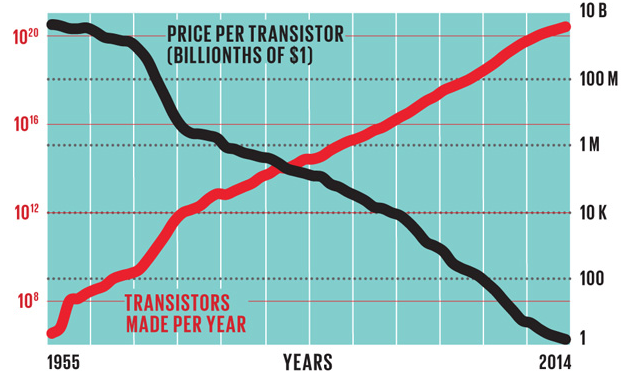
\includegraphics[clip=true, width=0.475\textwidth]{transistor}
	\caption{} \label{fig:transistor}
\end{figure}

Assuming an initial R\&D time frame of approximately 5 years for the first demonstration of a QMU, we further assume the same scaling in terms of the number of QMU's manufactured and illustrate the growth of the Sneakernet network though each state: 1) a large-scale, global authentication network, 2) a global key exchange network, and 3) a global one-time-pad encryption network. We also show a forth stage of the Sneakernet network: the ability to build a true Quantum Internet that connects large-scale, error-corrected quantum computing systems. Fig.~\ref{fig:QMU} illustrates network volume extrapolated using the same scaling as Fig.~\ref{fig:transistor} (in terms of the total number of QMU's manufactured after 2023) for the next 50 years. 

\begin{figure}[htbp!]
	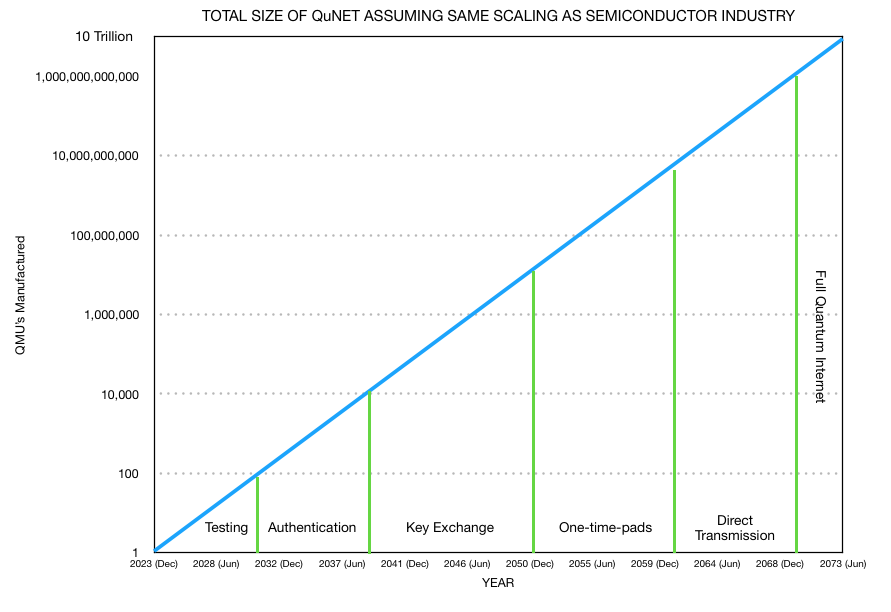
\includegraphics[clip=true, width=0.475\textwidth]{QMU}
	\caption{} \label{fig:QMU}
\end{figure}

If a similar trend line is followed, approximately ten trillion QMU's can be manufactured by 2073. This is an astronomical figure for active quantum devices; and it would also be more than sufficient to construct multiple, large-scale quantum computing systems capable of executing any large-scale algorithm that has ever been developed. But keeping our discussion limited to the communications space, the Sneakernet system is, as we have said, designed to incorporate new QMU's as they become available, rather than replacing them. So the total size of the network is cumulative. 

How such a network will be used is less clear. As noted above, we can make the following arguments as to when a particular application `comes online'
\begin{itemize}
\item Authentication tokens can come online once the number of QMU's $> 1\times 10^2$. 
\item Key exchange can come online once the number of QMU's $> 10\times 10^3$.
\item One-time-pads can come online once the number of QMU's $> 50\times 10^6$. This assumes voice communications using the 600 bps NATO standard STANAG-4591 vocoding technique with a cumulative total of 10 hours of communication that needs to be encoded using QuSTICKS.
\item Direct coupling of fully error-corrected quantum computers at a MHz logic-gate rate once the number of QMU's $> 10\times 10^9$. 
\item Large-scale quantum internet once the number of QMU's $> 1\times 10^{12}$.
\end{itemize}

Between 100 and 10,000 QMU's, the network can expand into a network consisting of 100 separate authentication links, with each link implemented at arbitrary distance scales. These separate links could be deployed between the same two parties (increasing the speed of a single link) or it could be spread out over multiple locations. How the network is configured and re-configured is completely at the discretion of whoever owns or controls the physical QuSTICKS. 

Once a total of 10,000 QMU's have been manufactured, the operator of the QuNET may choose to re-task \textit{all} the QMU's then deployed to form a single link dedicated to key exchange for symmetric encryption protocols such as AES. Once this is achieved, the process starts again. At this point the network can become a hybrid of both key exchange and authentication, with resources deployed depending on need. The expansion process continues using these two protocols until one-time-pad quantum encryption becomes feasible for data transmission of significant volume (at approximately 50 Million QMU's). At each stage of the QuNET expansion, resources can be dynamically redesigned to support whatever protocols are both possible (given the total number of units in the field) and what is desired by whomever controls the physical QuSTICK units. 

Once the number of QMU's exceeds the number needed to connect together fully error-corrected quantum computing systems, the network will continue to expand to encapsulate all the sub-protocols, completing the transition to a multi-purpose Quantum Internet. 

Our extrapolations based upon the historical evolution of the classical semiconductor industry is extremly optimistic; but given the design of a particular underlying technology, once a single QMU chip-set can be fabricated at low enough cost, expansion of the network becomes purely a function of how quickly high volume manufacturing can be developed and how much per-qubit costs can be reduced as that manufacturing infrastructure becomes more advanced. As with classical storage memory, requiring petabytes or exabytes of cheap, stable memories may have seemed completely unrealistic in the 1940's or 1950's but continual development of the technology has now made that that level of classical storage routine.

\subsection{Revisiting the criticisms from GCHQ}

Now that we have described the structure and operation of a Sneakernet based communications system, let us revisit some of the criticisms of the GCHQ (the UK's Government Communications Headquarters office) mentioned earlier in using Quantum Key Distribution (QKD) to secure classical communications channels. 

\textbf{QKD protocols address only the problem of agreeing on keys for encrypting data. Ubiquitous on-demand modern services, such as verifying identities and data integrity, establishing network sessions, providing access control, and automatic software updates, rely on authentication and integrity mechanisms (e.g. digital signatures) as well as encryption.}

As we have discussed, key distribution is only one protocol in a larger stack of applications of a Sneakernet network. The network can be used for authentication and session integrity by using shared entanglement between two parties to violate Bell inequalities; and the portability of the QuSTICK system allows for these authentication channels to be set up wherever physical access to transport is available.

\textbf{The two major functional limitations of commercial QKD systems are the relatively short effective range of transmission, and the fact that BB84 and similar proposals are fundamentally point-to-point protocols. This means that QKD does not integrate easily with the Internet or with the mobile technologies, apps and services that dominate public and business life today.}

This system is designed from the ground up to be functional over global distances. It doesn't need extensive infrastructure along the communications channel and can leverage classical transport mechanisms that are already available, efficient and ubiquitous. 

While we have illustrated much of the function of the Sneakernet system through point-to-point protocols between two parties, the design is a fully-formed quantum network. Entanglement can be distributed and shared between an arbitrary number of parties and more complex protocols, such as secret sharing or distributed communication/computation, can be performed. In the context of QKD, we do not utilise the point-to-point protocol of BB84. Instead we base QKD protocols on the more advanced Ekert-91 (which utilises two properties of entanglement, the perfect correlation of measurements made by Alice and Bob as well as the ability to detect eavesdropping by noting disturbances in the quality of that correlation). A Sneakernets ability to distribute, share and maintain entanglement on global distances makes Ekert-91 practical for real-world cryptography for the first time.

\textbf{Hardware is expensive to obtain and maintain. Unlike software, hardware cannot be patched remotely or cheaply when it degrades or when vulnerabilities are discovered.}

The Sneakernet network is built from the QMU chip sets and the QuSTICK devices. These devices are ideally designed to be cheap and to be mass manufactured, with network capabilities increasing as more and more units are produced. One of the major benefits to this system is that we can easily replace/repair or augment QuSTICKS within the network to fix potential vulnerabilities in the future or to simply fix faulty units. Unlike infrastructure-intensive quantum communication systems (such as quantum repeater networks or satellites), we have trivial access to each physical device within the network, and they can be repaired or replaced as simply as a non-functional hard-drive in a classical Sneakernet communications channel. Patching hardware remotely is not required, as the hardware itself is easily portable. Hence, if repairs or patches are needed, QuSTICK units can be rotated in and out of the larger network and then immediately redeployed in the field without significantly affecting the performance of the network. Once large volumes of QuSTICKs are deployed in the network, regular servicing and repairs of individual units will be background noise to overall network performance.  

\textbf{Any real-world QKD system will be built from classical components, such as sources, detectors and fibres, and potentially ancillary classical network devices, any one of which may prove to be a weak link. A number of attacks have been proposed and demonstrated on deployed QKD systems that subvert one of more of these hardware components, enabling the secret shared key to be recovered without triggering an alarm.}

Sources, detectors and fibres are not components of the Sneakernet system. The integrity of the network rests with the functional integrity of individual QuSTICKs. As these units will be continuously moved, entangled locally, and then moved again, QuSTICKs can be tested and verified when the entanglement is initially prepared. Various unit testing can be performed between two QuSTICKs at home base to ensure quantum integrity of the system before they are ever deployed in the field. Compromised units can be removed from the network or returned for a complete rebuild and redeployment. Any units that become compromised in the field will be detected through the entanglement links that were initially prepared when QuSTICKs were present at home base. As no further entanglement operations are performed between QuSTICK units \textit{after} they have been locally entangled and verified, points of failure (where security could be affected) are drastically reduced. 

\textbf{Denial of service (DoS) attacks that interfere with the paths carrying the QKD transmissions also seem potentially easier with QKD than with contemporary Internet or mobile network technologies. Since QKD devices typically abort a key establishment session when they detect tampering, this makes it difficult to recommend QKD for contexts where DoS attacks are likely to be attempted.}

As we have mentioned, denial of service attacks require an actual physical QuSTICK to be compromised. For an effective denial of service attack to be launched against the entire network, an adversary would have to steal or physically compromise \textit{every} QuSTICK unit one of the parties possesses -- a much more difficult thing to do than simply cutting an optic fibre link or jamming the transmission of photons. If only a subset of QuSTICKS are stolen or otherwise compromised, network performance will decrease, but provided there are at least two uncompromised units somewhere, a viable entanglement connection will exist. 

\subsection{A vision for the future: Creating a QuNET quantum internet}

The physical QMU resources needed to connect together fully error-corrected quantum computing systems would only be about an order of magnitude higher than using quantum methods to directly transmit encrypted or unencrypted classical data. A fully functional Quantum Internet (that is, a network with the ability to provide quantum communication channels between large-scale, error corrected quantum computers) requires the following:
\begin{itemize}
\item Transcontinental communication links spanning distances anywhere up to 10,000km.
\item A high speed network spanning those distances for $>$ THz operational speeds.
\item End-to-end error rates of $10^{-10}$ or lower.
\end{itemize}

Two ideas for constructing such worldwide quantum communication networks have received extensive theoretical examination and experimental demonstration: 1. Quantum repeater systems. 2. Quantum-based satellite communications. However, both approaches run into significant practical limitations.

High-speed quantum repeater networks only exist for \textit{theoretical} transmission rates of about 1-10 MHz and require repeater stations every 20 to 50 km. This upper limit to repeater station separation is necessitated by the loss rates of current optic fibre technology. It is unclear if that range can ever be extended. An associated problem with the small separation distances of quantum repeater stations is the difficulty of deploying networks across oceans or otherwise inhospitable environments. Quantum repeaters are small-scale quantum computers, consisting of thousands of qubits and associated control infrastructure. This requirement currently precludes their deployment at high densities across the planet. 

Regarding satellite technology, there has been significant experimental progress, with entanglement-based satellite platforms deployed by the Chinese, as well as proof-of-principle payloads deployed by the Singaporeans, Japanese and Austrians. These platforms are not designed for general purpose quantum communications. They are built for QKD applications, which do not have the stringent constraints listed above. 

While fully error-corrected, high bandwidth, and low error-rate satellite systems have not received significant theoretical attention as yet, we can safely assume that such technology \textit{could} be built and deployed. However, deployment and maintenance costs, bandwidth sufficient for fully error-corrected communications channels, and the infrastructure associated with receiving stations represent very big hurdles to overcome when utilising space based platforms as backbones to a Quantum Internet. 

QuSTICK-based quantum networks can satisfy the constraints noted above as well as address the issues associated with quantum repeaters and satellite communication systems. Initial analysis shows that $>$ THz transpacific networks can be realised in a systems of moderate physical speed and size, provided that the cost per physical qubit is low enough. Beyond the challenge of simply building a sufficient number of QuSTICKs (a challenge that is common for any hardware company targeting large-scale quantum computing platforms), there is no additional hardware development work needed to realise a global network. The only additional infrastructure needed by a global QuSTICK network is traditional global shipping channels that already exist. 

Prototype quantum communication networks using Sneakernet principles and QuSTICKs will first be demonstrated at much shorter ranges and at slower communication rates. Scaling up to higher fidelity, higher speed, and longer ranges is conceptually straightforward. Additionally, communications channels do not influence infrastructure development. Building a quantum communications system between Tokyo and Osaka is no different to building a communications system from Japan to Australia. 

Fig.~\ref{fig:link} illustrates the performance of a single link based on physically transporting QuSTICK units on cargo containers, over a distance of 10,000km with a link fidelity of 99.99\% as a function of the density of physical qubits inside each QMU. These are only back of the envelope calculations, but does illustrate that overall QMU density and number of units is the only impediment to achieving truely global link distances at ultra-high fidelity at bandwidths that approach what is currently possible in classical fibre optics communications. No other system proposed can scale to this level.
 
\begin{figure}[htbp!]
	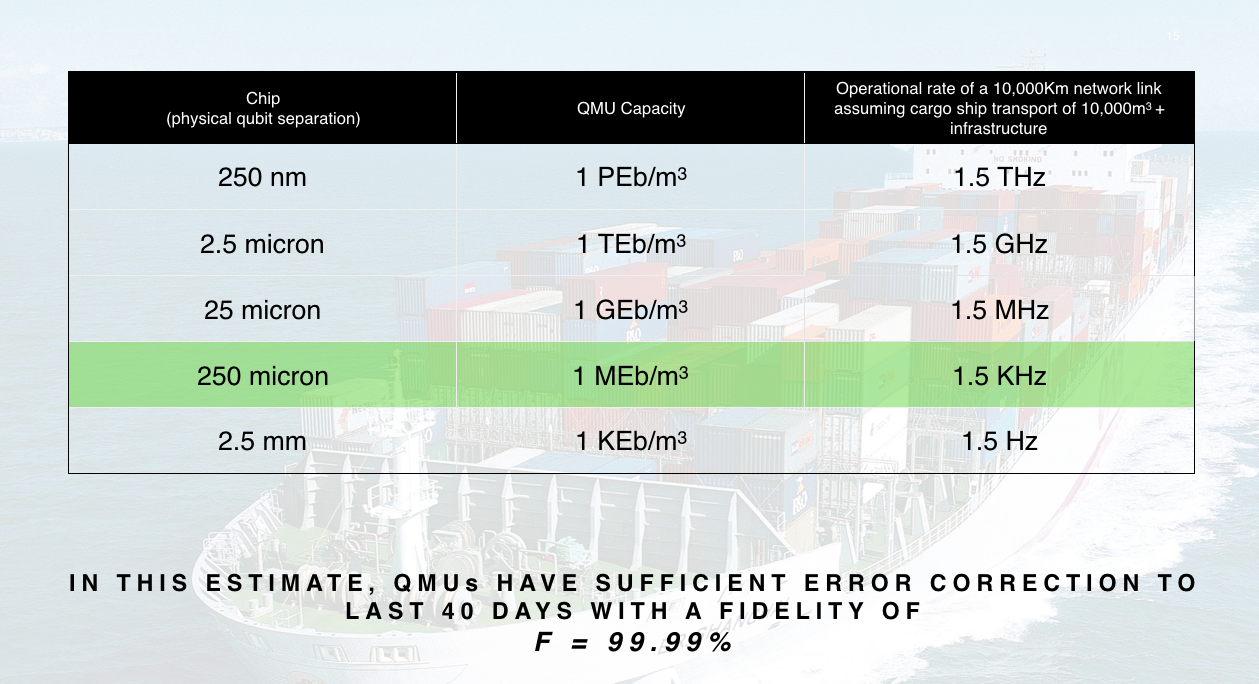
\includegraphics[clip=true, width=\columnwidth]{link}
	\caption{} \label{fig:link}
\end{figure}

While many of the other core technologies for quantum communications (satellites, fibre, free-space) can be used to augment secondary and tertiary communication links appropriate to the applications needed, Sneakernet based communication networks appear to be the best approach to form the major high-bandwidth truck lines of the future. 

\bibliography{sample}

\end{document}